% Meyer: Ergebnisse reflektieren, Diskussion (Titel: Test und Diskussion der Ergebnisse oder zwei Hauptkapitel)

Nach Abschluss der Realisierung aller zuvor erstellten Planungen, folgt nun im letzten großen Schritt die Auswertung der erzielten Ergebnisse. Ein entscheidendes Ziel dieser Arbeit ist das Finden einer möglichst guten Optimierung zu der zu Beginn gesetzten Problemstellung. Zweck dieses Abschnittes ist es nun also, zu zeigen ob bzw. wie gut dieses Ziel erreicht wurde. Dazu werden zunächst quantitative Auswertungen anhand wichtiger und auch im folgenden bestimmter Metriken angestellt. Anschließend folgt dann eine qualitative Diskussion mit Bezug auf das gesteckte Ziel.

Um zunächst einmal einen Eindruck der Effektivität und der Ergebnisse der einzelnen Algorithmen zu erhalten, sollen diese zunächst getrennt voneinander zahlenmäßig ausgewertet werden. Dies ist auch sinnvoll, da das Vorgehen und die Ergebnisse durchaus unterschiedlich sind und sich nicht sofort und direkt miteinander vergleichen lassen.

\subsection{Auswertung Algorithmus 1 (RS)}

Um einen guten Vergleich und eine Bewertung der verschiedenen umgesetzten Algorithmen anstellen zu können, wurden im folgenden verschiedene interessante Metriken erarbeitet. Es folgt jeweils eine Beschreibung von passenden Testszenarios zur Ermittlung der Metriken und deren zur Auswertung. Anschließend werden die auf diesem Weg entsprechende Graphen für jeden Algorithmus erzeugt und gegenübergestellt.

\subsubsection{Aufbau der Testszenarien}

Die Tests sehen für alle folgenden Testfälle eine Gegenüberstellung der Ausgangssituation vor der Optimierung mit jeweils optimierten Ergebnissen vor. Dafür wird für alle Testfälle eine gleichbleibende Menge von verfügbaren Ressourcen angenommen, welche auf Erfahrungswerten zu benötigten Ressourcen basiert. Dies wäre auch ein nötiges Vorgehen, um am realen Terminal eine sinnvolle Auslastung zu erzielen. Dort wird die Verfügbarkeit aber möglicherweise je nach Personalverfügbarkeit (aus Krankheit, Urlaub etc.) oder Maschinenverfügbarkeit (durch Wartungen, Reparatur etc.) schwanken. Solche besonderen Szenarien werden in späteren Testfällen genauer betrachtet. Zunächst ist es aber der beste Weg, gewöhnliche Szenarien und Abläufe zu vergleichen. Betrachtet werden in allen Tests die zuvor implementierten Verfahren \glqq{}Shortest Job Next\grqq{} (SJN), \glqq{}Most Idle Time\grqq{} (MIT) und \glqq{}First come, first served\grqq{} (FCFS).

Mit folgender Liste von Ressourcen wurde jeweils gearbeitet:
\begin{itemize}
    \item 2x Gabelstapler (Forklift)
    \item 1x Kran (Crane)
    \item 2x Einweiser (Guide)
    \item 2x Fahrer (Driver)
    \item 1x Greifstapler (Reachstacker)
    \item 2x Ketten (Chains)
\end{itemize}

Die Slotgröße wurde in der Regel auf 180 Minuten, also 3 Stunden festgelegt.

Die Listen von verarbeiteten Avisierungen wird für alle Szenarien mit der eigens entwickelten Methode \textit{generateRandomAdvices()} generiert. Sie ermöglicht auch eine Generierung mit ungleicher Verteilung der Abfertigungskategorien der LKW. Für die meisten Testszenarien wird hier eine an die reale Verteilung angelehntes Verhältnis von 2:2:2:1 für LIFT\_CHAINS zu LIFT\_FORKS zu SELF\_DRIVING zu CONTAINER gewählt. \todo{Beibehalten, Quelle woher der Wert kommt}

Die Liste der gebuchten LKW real, wie auch in diesen Tests sehr zufällig. Um das Verhalten und die Streuung der Ergebnisse über viele Durchläufe vergleichen zu können, werden daher alle Werte 100 Mal berechnet und immer die Durchschnittswerte bzw. eine Standardabweichung gezeigt. 

\subsubsection{Testszenario 1: Verhalten mit unterschiedlicher Anzahl von LKW}

Um die Verbesserung durch die Algorithmen zu zeigen, werden die beschriebenen Durchläufe jeweils mit identischen Eingangsparametern, einmal mit dem eigens entwickelten \textit{UnoptimizedScheduler} und einmal mit den jeweiligen Optimierungsalgorithmen durchgeführt. Verglichen werden soll zunächst das Verhalten bei steigender Anzahl von avisierten LKW. Jeder Algorithmus wurde dafür mit einer zufällig generierten Liste von LKWs ausgeführt, wobei die Anzahl der LKW in dieser Liste schrittweise von 1 auf 100 \todo{Warum 100 erklären} erhöht wurde. Da die Ladung der LKW in Realität kaum vorhersehbar und zufällig ist, was auch hier im Test durch eine zufällige Generierung der Eingangsdaten nachgestellt wurde, wird jeder dieser Schritte 100\todo{Warum 100 erklären; 100 auch bei anderen Szenarien einfügen...} Mal mit einer unterschiedlichen Eingangsliste durchgeführt. So ist es möglich, in der nun folgenden Auswertung Durchschnittswerte zu bilden und insbesondere auch Streuungen näher zu betrachten.

Die Werte zu den folgenden Graphen wurden durch die implementierten Testläufe der Testklasse \textit{NumberOfTrucksTest} ermittelt. Alle nachfolgend erklärten Berechnungen und die Erzeugung der Graphen wurden mit dem R Skript \textit{rsNumberOfTrucks.R}\todo{Pfad etc} erzeugt.


\textbf{Verbesserung der Anzahl abgefertigter LKW}

Ziel des gesamten Optimierungsaufwands war es, avisierte LKW effektiv auf einen Slot zu verteilen, sodass möglichst viele LKW abgearbeitet werden können, bzw. dass möglichst wenig Leerlaufzeiten entstehen. Dargestellt wird hier zunächst die prozentuale Verbesserung der Anzahl der erfolgreich eingeplanten LKW (Berechnung siehe Formel \ref{eq:schedJobImpr}) gegenüber der Gesamtanzahl von Buchungen. Ein prozentualer Wert des optimierten Wertes gegenüber dem Unoptimierten gibt in diesem Fall den besten Überblick, wie viel Verbesserung erreicht werden konnte. Die totale Anzahl von LKW kontinuierlich, die Verbesserung wäre hier schwerer zu erkennen.

\begin{equation} \label{eq:schedJobImpr}
schedJobImpr = \left(\dfrac{100}{uScheduledJobs} * oScheduledJobs\right) - 100
\end{equation}

In den Graphen (siehe Abb. \ref{fig:evalAnzahlLkw}) dargestellt wird dabei jeweils der Durchschnittswert über alle 100 Durchläufe, sowie dessen jeweilige einfache Standardabweichung, um ein Maß für die Streuung zu erhalten.

\begin{figure}[H]
\centering
\begin{subfigure}{.495\textwidth}
  \centering
  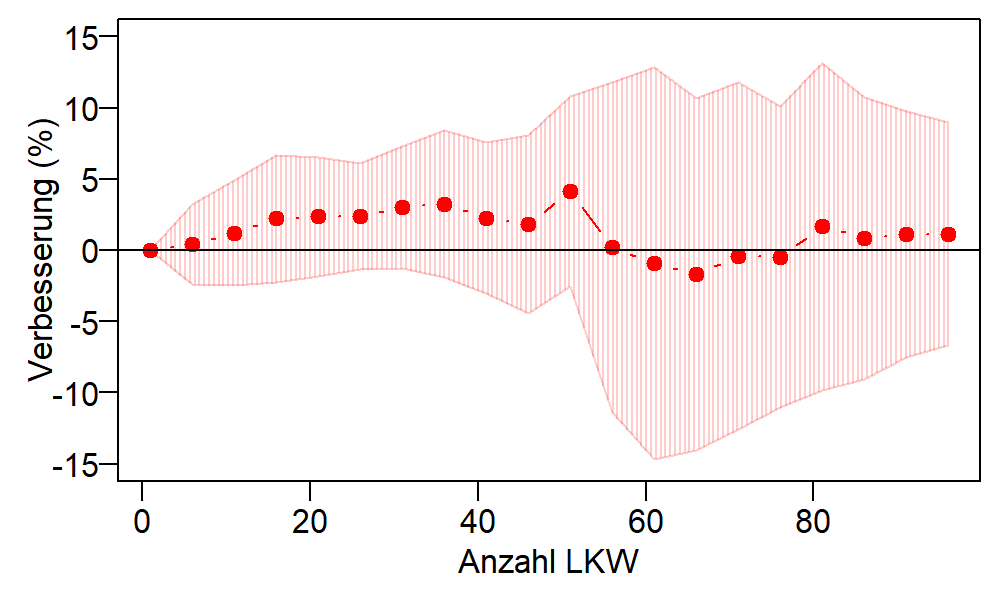
\includegraphics[width=\linewidth]{images/graphs/rsNumberOfTrucksSjn_AnzahlAbgefertigt.png}
  \caption{Shortest Job Next}
  \label{fig:eal1}
\end{subfigure}
\begin{subfigure}{.495\textwidth}
  \centering
  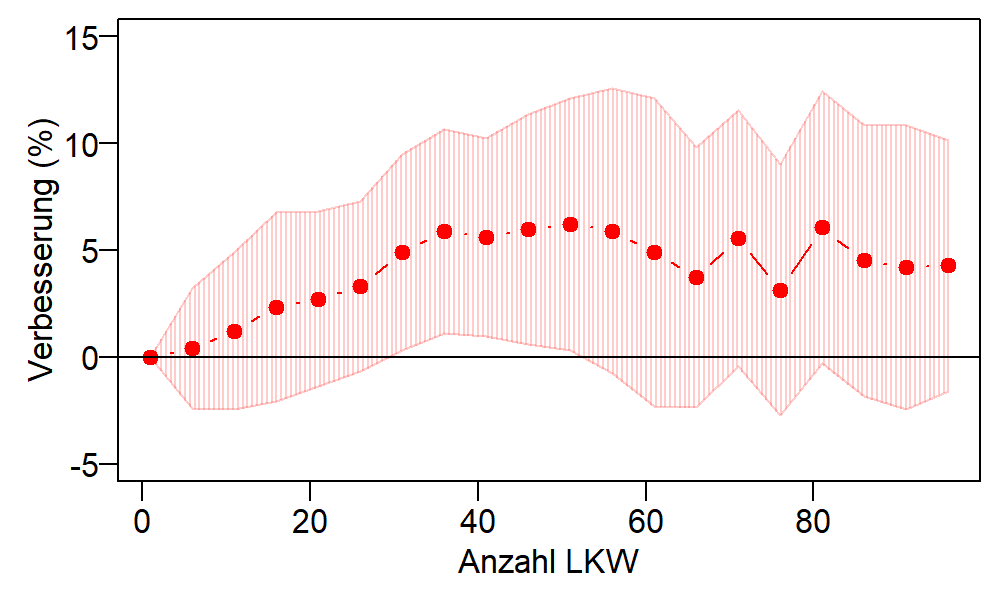
\includegraphics[width=\linewidth]{images/graphs/rsNumberOfTrucksMot_AnzahlAbgefertigt.png}
  \caption{Most Idle Time}
  \label{fig:eal2}
\end{subfigure}

\begin{subfigure}{.5\textwidth}
  \centering
  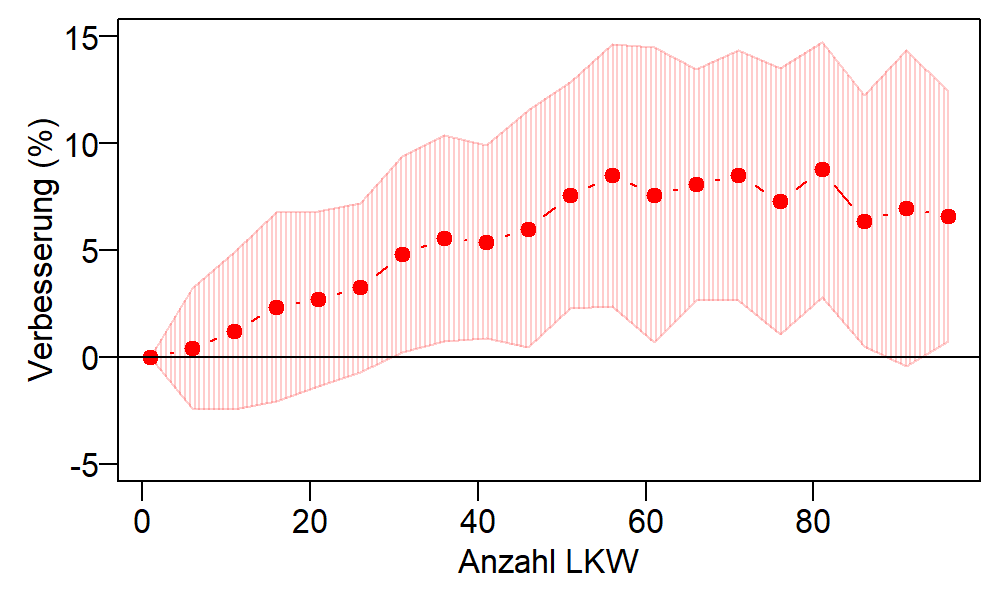
\includegraphics[width=\linewidth]{images/graphs/rsNumberOfTrucksFcfs_AnzahlAbgefertigt.png}
  \caption{First come, first served}
  \label{fig:eal3}
\end{subfigure}

\caption{Verbesserung der Anzahl abgefertigter LKW}
\label{fig:evalAnzahlLkw}
\end{figure}

Was zunächst einmal bei allen Algorithmen auffällig ist, ist dass die Standardabweichung, also die Streuung der Werte sehr hoch ist. Hier ist jeweils die einfache Standardabweichung dargestellt, d.h. geht man von einer Normalverteilung der Werte aus, so liegen in den rot schraffierten Bereichen 68\% der Werte. Eine doppelte Standardabweichung mit 95\% der Werte würde also bei allen Algorithmen im negativen Bereich liegen. Kein Algorithmus garantiert also eine Verbesserung der Werte. Ebenfalls ist bei allen Graphen eine stark sichtbare Veränderung des Anstiegs zwischen 40 und 60 LKW zu erkennen. Dies dürfte etwa die Grenze sein, bei der der 180 Minuten Slot vollgefüllt ist. Bis dort hin bleibt so viel Leerlauf, dass die meisten LKW noch eingeplant werden können, ab dann können die meisten neuen LKW nicht mehr eingeplant werden. Alle Graphen zeigen auch bis etwa 30 LKW eine ähnlich starke Verbesserung von ca. 4-5\%, was darauf zurückzuführen ist, dass in diesem Bereich immer nahezu alle LKW eingeplant werden können und keiner verschoben werden muss.

Auffällig in Graph \ref{fig:eal1} für das Shortest Job Next Verfahren ist allerdings, dass es eine deutlich geringere Verbesserung bei insgesamt größerer Streuung gibt. Bis der Slot bei etwa 50 LKW gefüllt ist, gibt es durchschnittlich eine leichte Verbesserung bis zu etwa 3\%. Die Streuung ist dabei sogar leicht geringer als bei den anderen Algorithmen. Danach fällt die Verbesserung allerdings stark ab und pendelt um 0 herum, teilweise sogar leicht ins negative bei extremer Streuung. Schaut man sich beispielhaft eine grafische Darstellung der Verteilung an (siehe Abb. \ref{}\todo{Beispiel einfügen}), so fällt auf, dass durch die Verplanung der kurzesten Aufgaben am Anfang eine starke Ungleichverteilung entsteht. Zumindest bei den hier gewählten Ladezeiten haben immer die gleichen Abfertigungskategorien auch die kürzesten Ladezeiten, sodass immer die gleichen Ressourcen genutzt werden und im Anschluss andere kaum mehr verplant werden können, weil sie oft parallel mit bereits verplanten Ressourcen vorkommen.

Im Planungsverfahren mit der meisten Leerlaufzeit (siehe Graph \ref{fig:eal2}) lässt sich eine deutlichere Verbesserung erkennen. Bis zur Füllung des Slots bei etwa 40 LKW gibt es eine kontinuierliche Verbesserung bis zu ca. 5\%, bei moderater Streuung. Anschließend pendelt sich die Verbesserung bei 5\% ein, bei allerdings deutlich steigender Streuung. Die anfängliche Steigung dürfte damit zusammen hängen, dass es mit wenigen LKW einfach auch nur möglich ist eine geringe Verbesserung zu erzielen. Je mehr LKW kommen, desto mehr Potenzial kann auch ausgeschöpft werden.

Bei der first come, first served Verteilung (siehe Graph \ref{fig:eal3}) ergibt sich ein sehr ähnliches Bild wie in Graph \ref{fig:eal2}. Bis etwa 40 LKW sind die Steigung und auch die Streuung sehr ähnlich. Allerdings geht die Steigung hier noch bis eta 50 LKW und 7-8\% Verbesserung weiter. Erst dann stagniert diese ebenfalls auch etwa gleichbeibender Höhe und deutlich steigender Streuung.

Bezüglich der Anzahl der möglichen Abfertigungen lässt sich aus dieser Betrachtung schließen, dass die Algorithmen MIT und FCFS für den allgemeinen Fall deutlich besser geeignet sind. Die große Streuung zeigt allerdings auch, dass es sehr große Unsicherheiten bei allen Algorithmen gibt. Dies dürfte vor allem mit der Zufälligkeit der Eingabewerte zusammenhängen. Wenn kaum etwas über die Verteilung der ankommenden LKW bekannt ist, ist es sehr schwierig einen spezialisierten Algorithmus zu finden. Somit kann nur auf allgemein funktionierende Verfahren zurückgegriffen werden, welche dann in der Regel auch Verbesserte Werte liefern. Was allerdings positiv zu bemerken ist, ist dass genau der Wendepunkt zu dem die Slots gefüllt sind, auch der Hochpunkt der Verbesserung ist. Es ergibt aus dieser Betrachtungsweise somit kaum Sinn, Überbuchungen und anschließende Verschiebung einiger LKW in andere Slots vorzunehmen, da es kaum noch Verbesserung bei der Anzahl der verarbeiteten LKW gibt.


\textbf{Verbesserung der Leerlaufzeiten der Ressourcen}

Die Leerlaufzeit der Ressourcen ist, wie erwähnt, ebenfalls von Bedeutung. Je weniger ungenutzte Leerlaufzeit eine Ressource innerhalb des Slots hat, desto mehr wird sie produktiv und wirtschaftlich sinnvoll eingesetzt. Auch hier ist als relatives Maß die prozentuale Verbesserung zwischen den jeweils unoptimierten und optimierten Zeiten aufgetragen. Berechnet wurden diese nach den Formeln \ref{eq:idleImpr} und \ref{eq:idleBestJobsImpr}. Da die Leerlaufzeit bereits in Prozent gespeichert wird, reicht hier die Darstellung der Differenz, um die Verbesserung zu sehen.

\begin{equation} \label{eq:idleImpr}
idleImpr = uIdleTotal - oIdleTotal
\end{equation}
%\begin{equation} \label{eq:idleCompleteImpr}
%idleCompleteImpr = uIdleComplete - oIdleComplete
%\end{equation}
\begin{equation} \label{eq:idleBestJobsImpr}
idleBestJobsImpr = uIdleBetweenJobs - oIdleBetweenJobs
\end{equation}

Die Graphen stellen hier jeweils die Verbesserungen der gesamten Leerlaufzeit, der Leerlaufzeit und die Leerlaufzeit zwischen den einzelnen Jobs dar.

\begin{figure}[H]
\centering
\begin{subfigure}{.495\textwidth}
  \centering
  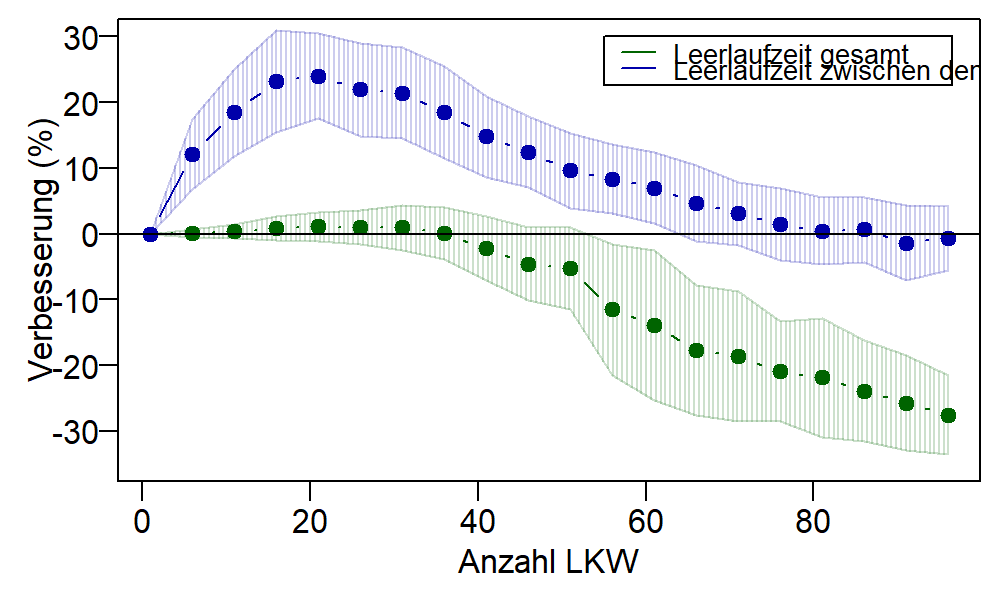
\includegraphics[width=\linewidth]{images/graphs/rsNumberOfTrucksSjn_Leerlaufzeit.png}
  \caption{Shortest Job Next}
  \label{fig:el1}
\end{subfigure}
\begin{subfigure}{.495\textwidth}
  \centering
  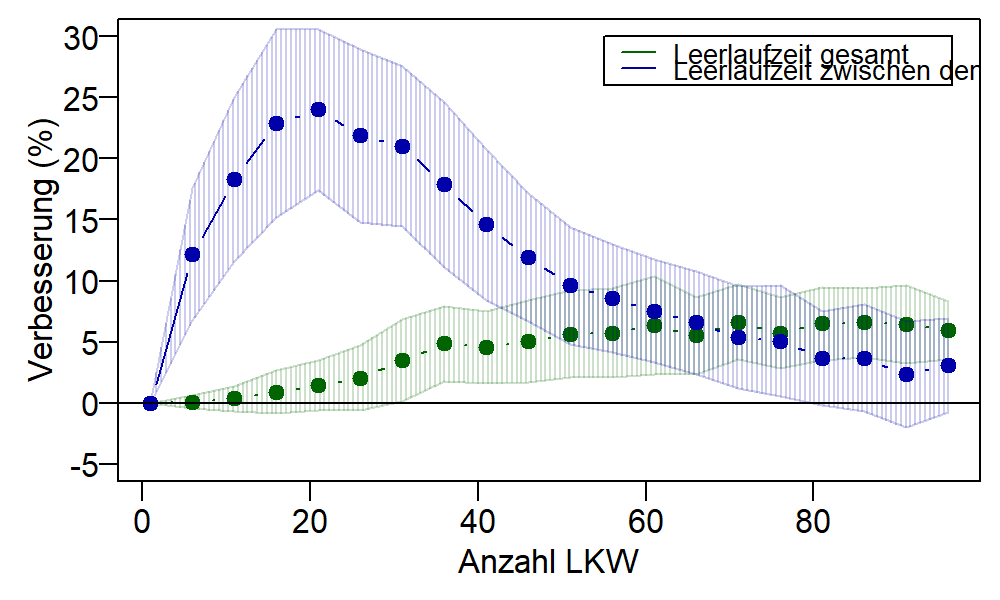
\includegraphics[width=\linewidth]{images/graphs/rsNumberOfTrucksMot_Leerlaufzeit.png}
  \caption{Most Idle Time}
  \label{fig:el2}
\end{subfigure}

\begin{subfigure}{.5\textwidth}
  \centering
  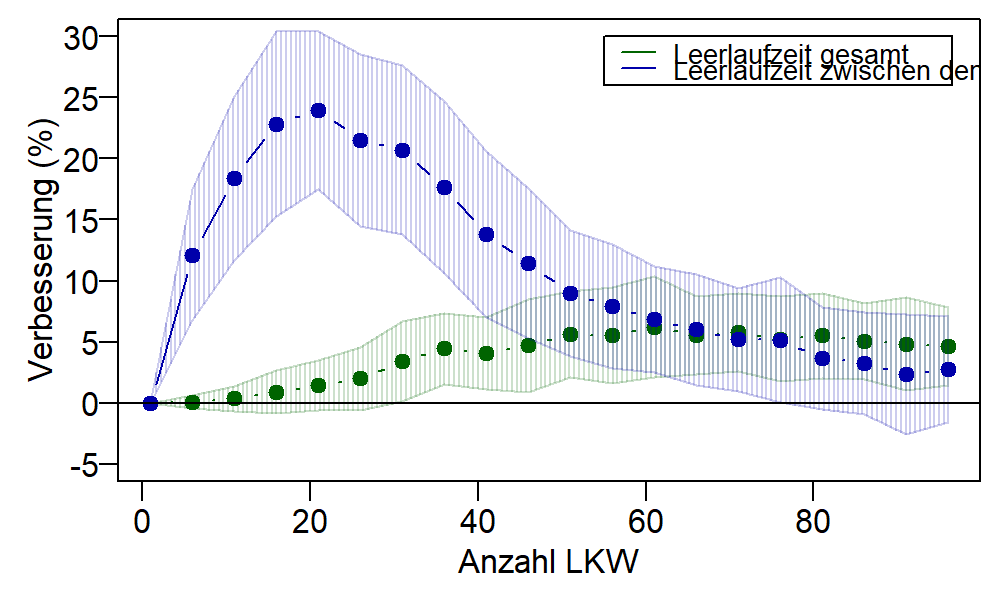
\includegraphics[width=\linewidth]{images/graphs/rsNumberOfTrucksFcfs_Leerlaufzeit.png}
  \caption{First come, first served}
  \label{fig:el3}
\end{subfigure}

\caption{Verbesserung der Leerlaufzeiten der abgefertigten LKW}
\label{fig:evalLeerlaufzeit}
\end{figure}

Mit Blick auf die Leerlaufzeiten lässt sich feststellen, dass die Streuungen hier zwar vorhanden, aber deutlich geringer sind. In den meisten Fällen ergeben sich so keine negativen Verbesserungen bzw. Verschlechterungen der Werte.

In Bezug auf die Leerlaufzeiten schneidet das SJN Verfahren allerdings auch nicht besonders gut ab (siehe Graph \ref{fig:el1}). Die Leerlaufzeiten zwischen den Aufträgen verzeichnen hier zwar eine deutliche Verbesserung von im maximalen Durchschnitt etwa 25\%. Auch die Standardabweichung bis etwa 50-60 LKW so gering, dass es hier so gut wie durchgängig Verbesserungen gegenüber dem unoptimierten Fall gibt. Die Gesamtleerlaufzeit über den Slot verbessert sich allerdings zu Beginn nur ganz minimal und dann zwar auch nur mit sehr geringer Streuung, allerdings verschlechtert sich diese nach dem Füllen des Slots sehr rapide bis zu etwa -25\% bei 100 LKW und einer größer werdenden Streuung. Erklären lässt sich dies in Kombination mit der Anzahl der abgefertigten LKW (siehe Graph \ref{fig:eal1}). Bis der Slot gefüllt ist, lassen sich unoptimiert wie optimiert so gut wie alle LKW unterbringen, somit ergibt sich dort wenig Vorteil bei der Leerlaufzeit. Danach allerdings werden im Durchschnitt gar keine zusätzlichen LKW eingeplant, dafür werden allerdings nach dem Shortest Job Next Prinzip nur die kurzen Aufgaben verplant und die langen fallen heraus und müssen verschoben werden. Insgesamt entsteht aber so eine geringere Auslastung der Ressourcen und somit eine deutliche Verschlechterung, die auch immer weiter ansteigt, je mehr kurze Aufträge es gibt.

Die Verfahren MIT und FCFS unterscheiden sich im direkten Vergleich nur sehr minimal (siehe Graphen \ref{fig:el2} und \ref{fig:el3}). Beide zeigen über den ganzen Zeitraum eine deutlich positive Verbesserung der Leerlaufzeit zwischen den LKW. Diese steigt bis im Durchschnitt etwa 25\% bei 20 LKW an und nimmt dann wieder ab. Um den Bereich zwischen 50 und 60 LKW, wo der Slot wieder komplett ausgefüllt wird, verlangsamt sich diese Abnahme, bleibt aber weiter positiv. Auch unter Berücksichtigung der Standardabweichung ist diese Verbesserung in nahezu allen Fällen positiv. Auch die Gesamtleerlaufzeit lässt eine gute Verbesserung erkennen. Bis etwa 6\% bei 60 LKW steigt diese Zeit bei beiden kontinuierlich an und hält sich dann auf etwa gleichbleibendem Niveau. Die Standardabweichung ist dabei zunächst sehr gering und wird dann bis zum höchsten Niveau immer größer. De größte Teil aller Werte liegt dabei aber immer noch im positiven Bereich, wenn auch deultich geringer als der Durchschnitt.

Schlussfolgern kann man aus dieser Betrachtung, dass das SJN Verfahren zwar für die Verplanung einzelner Ressourcen bezüglich der Leerlaufzeit Vorteile bringt, da die Zeiten zwischen den Ressourcen minimiert werden, über alle Ressourcen betrachtet ergibt sich allerdings kein Vorteil bzw. sogar ein starker Nachteil. Es werden nur kürzere und dabei aber auch nicht mehr Aufträge verplant. Dies bringt nicht nur hier Nachteile, die verschobenen Jobs müssen in späteren Slots zusätzlich eingeplant werden, was dort ebenfalls für große Schwierigkeiten und eine Ungleichverteilung der Auslastungen sorgen wird. Die beiden anderen Verfahren können dagegen allerdings den psoitiven Eindruck der vorherigen Auswertung bestätigen. Bei mehr eingeplanten LKW kann hier gleichzeitig eine geringere Leerlaufzeit verzeichnet werden. Der große Vorteil im Vergleich zu SJN dürfte sein, dass bei beiden Verfahren mehr oder weniger zufällig über alle Abfertigungskategorien hinweg aus den Aufträgen ausgewählt wird. Somit werden die Ressourcen im Schnitt gleichmäßiger ausgelastet und das strukturierte Vorgehen bei der Verteilung kann dann weniger Leerlauf schaffen und so zusätzliche LKW einsetzen.



\textbf{Verbesserung der Wartezeiten je LKW}

Ein Wert, welcher nicht direktes Ziel der Verbesserung war, aber dennoch interessant für eine nähere Betrachtung ist, ist die Entwicklung der Wartezeit der LKW. Lassen sich LKW schneller zu Beginn abarbeiten, kann dies ein Vorteil sein, da LKW Fahrer so nicht so lange ungenutzte Wartezeiten vor oder im Terminal haben und schneller für ihre Speditionen neue Aufträge bearbeiten können.

\begin{equation} \label{eq:avgWaitingImpr}
avgWaitingImpr = \dfrac{uAverageWaitingTime - oAverageWaitingTime}{uAverageWaitingTime} * 100
\end{equation}

\begin{figure}[H]
\centering
\begin{subfigure}{.495\textwidth}
  \centering
  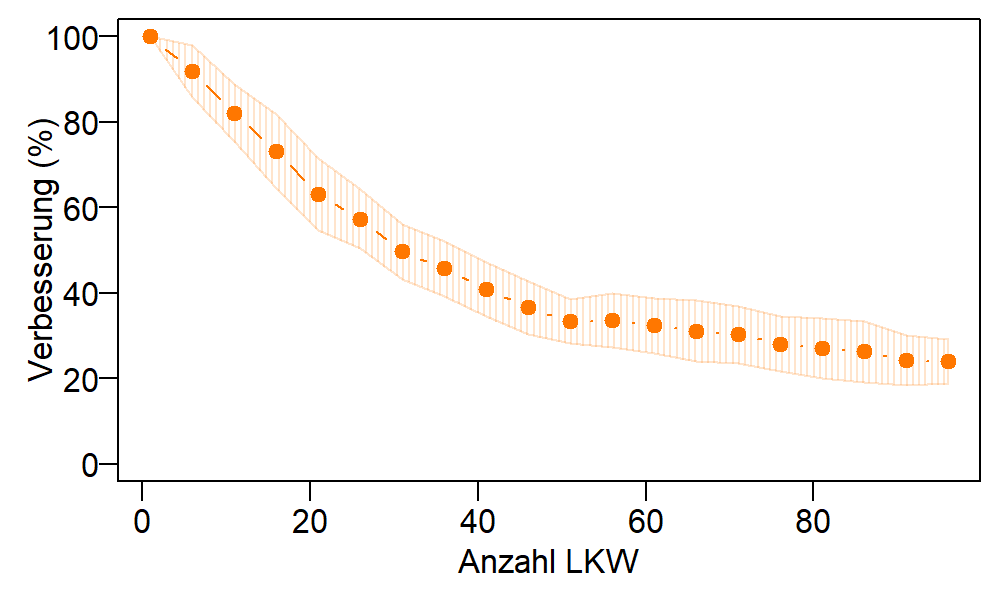
\includegraphics[width=\linewidth]{images/graphs/rsNumberOfTrucksSjn_Wartezeit.png}
  \caption{Shortest Job Next}
  \label{fig:ew1}
\end{subfigure}
\begin{subfigure}{.495\textwidth}
  \centering
  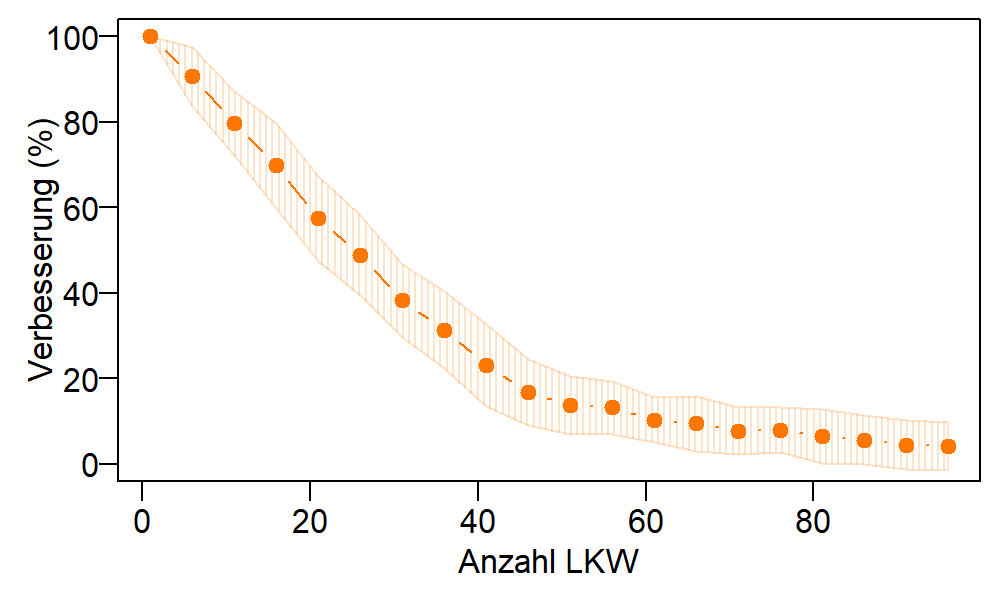
\includegraphics[width=\linewidth]{images/graphs/rsNumberOfTrucksMot_Wartezeit.png}
  \caption{Most Idle Time}
  \label{fig:ew2}
\end{subfigure}

\begin{subfigure}{.5\textwidth}
  \centering
  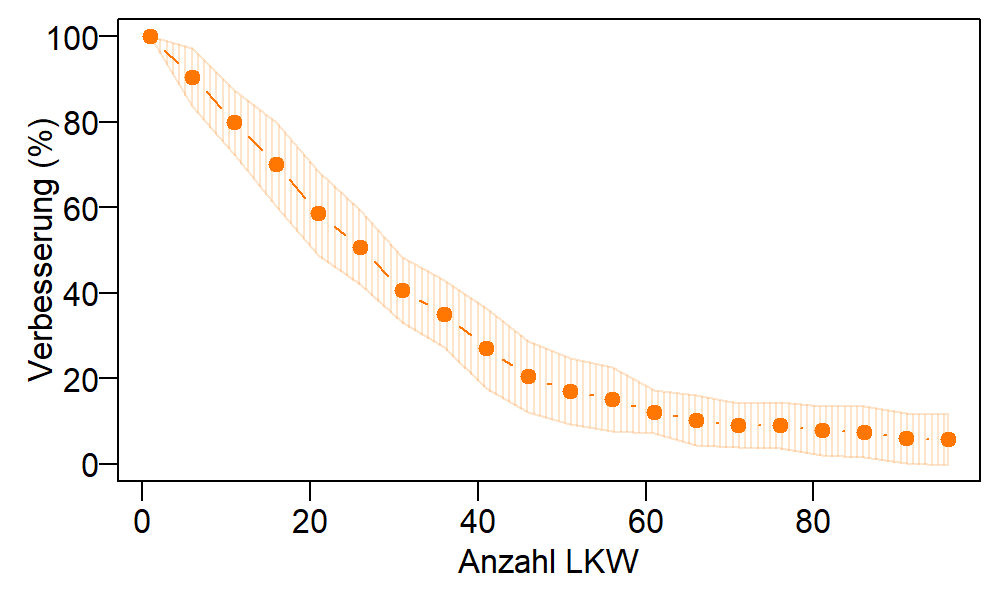
\includegraphics[width=\linewidth]{images/graphs/rsNumberOfTrucksFcfs_Wartezeit.png}
  \caption{First come, first served}
  \label{fig:ew3}
\end{subfigure}

\caption{Verbesserung der Wartezeit der abgefertigten LKW}
\label{fig:evalWartezeit}
\end{figure}

Bei den Wartezeiten ergibt sich ein etwas anderes Bild der betrachteten Verfahren. Alle beginnen bei einer Verbesserung der Wartezeit von 100\%, welche dann überall deutlich sinkt, bis zu dem Punkt wo wieder der gesamte Slot gefüllt ist. Ab diesem Punkt sinkt die Wartezeit überall weiter, allerdings deutlich langsamer. Auch die Streuung ist in diesem Fall sehr gering, sodass es keine Verschlechterungen der Wartezeit gibt.  Die anfänglich sehr große Verbesserung lässt sich darauf zurückführen, dass die LKW im unoptimierten Fall sehr zufällig verteilt über den gesamten Zeitraum des Slots ankommen. So wird jedes Planungsverfahren, welches die Aufgaben so früh wie möglich einplant, zunächst eine deutliche Verbesserung erreichen.

Auffällig ist vor allem, dass die Wartezeit den SJN Verfahrens (siehe Graph \ref{fig:ew1}) langsamer sinkt und sich auch am Ende noch auf einem Niveau von 30-40\% Verbesserung bewegt, während die anderen beiden Fälle (siehe Graphen \ref{fig:ew2} und \ref{fig:ew3}) wieder sehr ähnlich sind und gegen Ende nur noch eine Verbesserung von 10-20\% haben. Dies ist daraum zurückzuführen, dass das SJN Verfahren alle kurzen Aufgaben zuerst einplant, somit können schnell viele LKW abgearbeitet werden, was zu wenig Wartezeit führt. Spätestens, wenn der Slot komplett gefüllt ist und LKW verschoben werden müssen, wird sich der Vorteil dadurch relativieren, dass die verschobenen LKW mit langer Abfertigungszeit in anderen Slots untergebracht werden müssen und damit dort die Wartezeit negativ beeinflussen.

Insgesamt lässt sich aber festhalten, dass in allen Verfahren eine, wenn auch nicht immer allzu hohe Verbesserung erzielt werden kann. Dies war zwar nicht oberstes Ziel der Optimierung, ist allerdings ein schöner und für die LKW Fahrer und Speditionen vorteilhafter Nebeneffekt.



\subsubsection{Testszenario 2: Verhalten bei Überbuchung}

Ein weitere Betrachtungsweise der Algorithmen ist das Verhalten mit zunehmender Anzahl von Buchungen. In diesem Fall wird eine gleichbleibende Liste von Buchungen genutzt, welcher schrittweise LKW hinzugefügt werden. Dies simuliert, dass sich immer weitere LKW Fahrer einen Slot buchen. Interessant ist hier, wie viel Verbesserung sich erzielen lässt, wenn bis zur Auslastungsgrenze des Slots gebucht werden würde und alle weiteren, nicht mehr passenden LKW abgewiesen, bzw. diesen nur noch andere Slots zu Buchung vorgeschlagen werden. Dagegen wäre die Frage, wie viele Überbuchungen man zulassen könnte. Hier würden dann zunächst mehr LKW angenommen, als schaffbar sind. Der Planungsalgorithmus kann dann die für ihn passenden Buchungen nutzen und die restlichen in den nächsten Slot verschieben. Es wurden hier sehr ähnliche Berechnungen, wie im vorherigen Testszenario angewendet, auch hier wird ein Vergleich von simulierten, unoptimierten Zustand zu den Ergebnissen der verschiedenen Algorithmen vorgenommen.

Die Werte der folgenden Auswertung wurden durch die Testklasse \textit{OverfillTest} erzeugt. Alle anschließenden Berechnungen und Graphen sind mit dem R Skript \textit{rsOverfill.R}\todo{Pfad etc} berechnet worden.

Die Graphen (Abb. \ref{fig:evalOverfill}) zeigen in diesem Fall jeweils die absolute Anzahl an tatsächlich geplanten LKW im unoptimierten Zustand (blau) und im optimierten Fall (rot). So ist in hier deutlicher erkennbar, wann nicht mehr alle LKW eingeplant werden können, wann also Überbuchungen stattfinden müssten. Die diagonale Gerade mit einer Steigung von 1 zeigt dabei den Fall eines unbegrenzten Slots, sodass jeder LKW, welcher gebucht wurde auch verarbeitet werden kann. Im Verhältnis dazu wird auf der zweiten y-Achse die Verbesserung der Leerlaufzeit aufgetragen. Die Zeit zwischen den LKW in orange und die Gesamtleerlaufzeit in grün. Diese wurden wieder nach dem gleichen Weg wie im ersten Testszenario berechnet (siehe Formeln \ref{eq:idleImpr} und \ref{eq:idleBestJobsImpr}). So lässt sich ein direkter Vergleich anstellen, bei wie viel Buchungen die effektivste Ausnutzung des Slots erreicht wird.


\begin{figure}[H]
\centering
\begin{subfigure}{.495\textwidth}
  \centering
  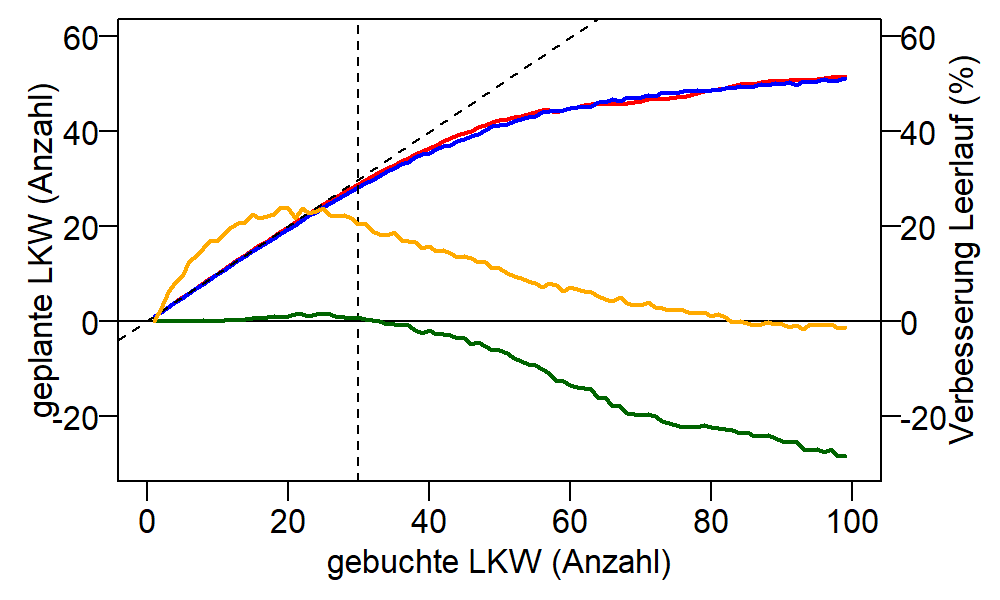
\includegraphics[width=\linewidth]{images/graphs/rsOverfillSjn.png}
  \caption{Shortest Job Next}
  \label{fig:eof1}
\end{subfigure}
\begin{subfigure}{.495\textwidth}
  \centering
  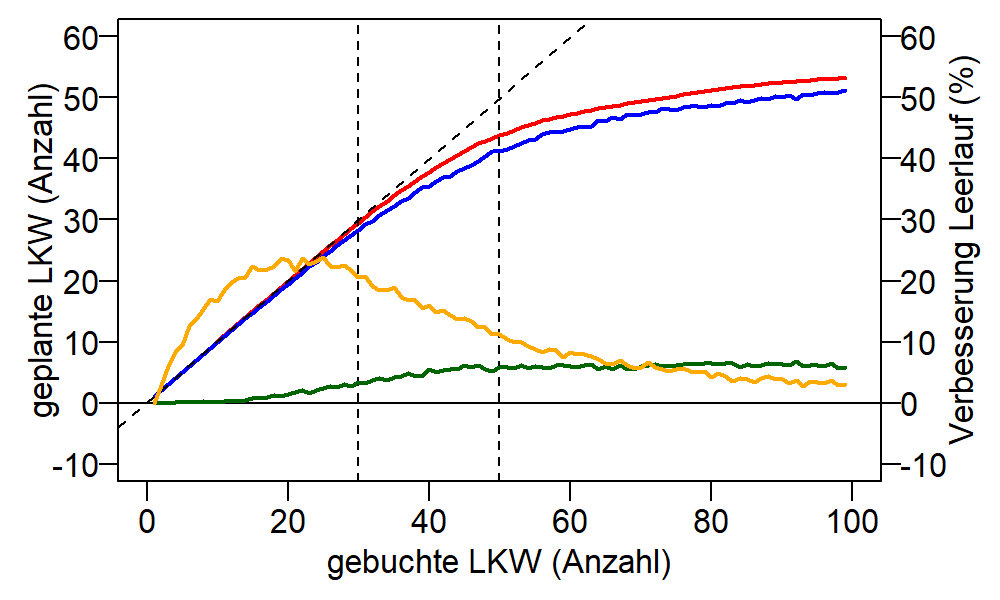
\includegraphics[width=\linewidth]{images/graphs/rsOverfillMit.png}
  \caption{Most Idle Time}
  \label{fig:eof2}
\end{subfigure}

\begin{subfigure}{.5\textwidth}
  \centering
  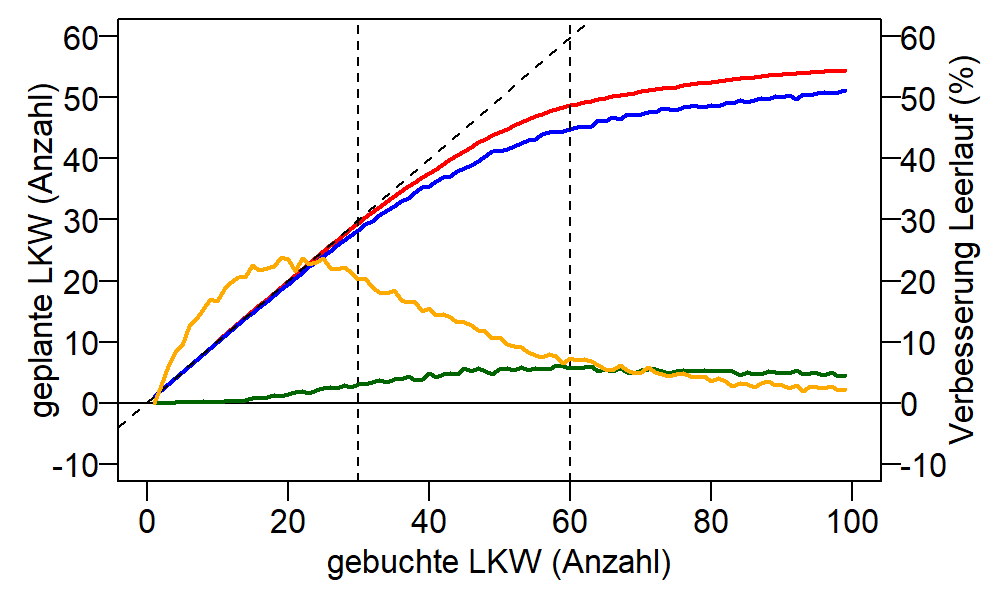
\includegraphics[width=\linewidth]{images/graphs/rsOverfillFcfs.png}
  \caption{First come, first served}
  \label{fig:eof3}
\end{subfigure}
\caption{Verhalten bei Überbuchung}
\label{fig:evalOverfill}
\end{figure}
\todo{Zuklein?, Legende?!}

Erkennbar ist zunächst einmal bei allen Darstellungen, dass überall die Anzahl der eingeplanten LKW bei etwa 30 anfängt, von der diagonalen für den unbegrenzten Slot abweicht. Dies ist also bei allen der Punkt, wo im Durchschnitt langsam nicht mehr alle LKW in den Slot passen. Verdeutlicht wird dieser Punkt in allen Graphen durch die erste senkrechte Linie.

Im SJN Verfahren (siehe Graph \ref{fig:eof1}) halten sich die beiden Anzahlen der eingeplanten LKW sehr nah beieinander, es gibt also im Durchschnitt kaum Verbesserungen oder Verschlechterungen. Die Gesamtleerlaufzeit verschlechtert sich ganz zu Beginn leicht und Verbessert sich dann bis zur markanten Grenze von 30 LKW leicht. Anschließend fällt sie rapide ab, wie es auch schon im vorherigen Szenario sichtbar war. Fängt man hier also an zu überbuchen, werden im Durchschnitt nicht mehr LKW abgefertigt, dafür steigt aber die Leerlaufzeit massiv. 

Auch in diesem Beispiel wiesen die Graphen der Verfahren MIT und FCFS (Abb. \ref{fig:eof2} und \ref{fig:eof3}) deutliche Ähnlichkeiten auf. Hier lässt sich allerdings ab 30 LKW ein größerer Anstieg der geplanten LKW im optimierten Fall erkennen, als es unoptimiert der Fall ist. Auffällig ist aber, dass die Steigung bei MIT schon bei etwa 50 LKW anfängt, deutlicher zu sinken, während es im FCFS Verfahren erst bei etwa 60 LKW der Fall ist (vgl. die zweite senkrechte Linie in den jeweiligen Graphen). Dies ist auch jeweils der Punkt, wo der Abstand zwischen der roten und der blauen Linie nicht mehr größer wird und somit auch kaum noch eine Verbesserung in der Anzahl der abgefertigten LKW stattfindet. Gleichzeitig ist dies auch der Punkt, an dem die Steigung bei der Verbesserung der Gesamtleerlaufzeit stagniert. Auch die Verbesserung Leerlaufzeit zwischen den den Aufträgen nähert sich ab da der Null an. 

Für die beiden Planungsverfahren MIT und FCFS kann man also festhalten, dass gewisse Überbuchung durchaus von Vorteil ist. Für den dreistündigen Slot, welcher ohne Überbuchung schon bei ca. 30 LKW gefüllt wäre, kann man durchaus eine Überbuchung im Bereich von 50-100\%, also insgesamt 45 bis 60 LKW zulassen. Dies führt zu einer deutlich optimierten Auslastung des Slots. Während im SJN Verfahren eine Verschiebung bedeuten würde, dass auch in nachfolgenden Slots eine Ungleichverteilung stattfinden würde, würde sich eine Verschiebung hier vermutlich nicht wirklich negativ auswirken. Da die Verteilung der Abfertigungskategorien, wie bereits festgestellt, ohnehin sher gleichmäßig ist, würde auch eine gleichmäßig durchmischte Liste verschoben. Darüber hinaus lässt sich eben bei einer Überbuchung eine deutlich verbesserte Auslastung und verringerte Leerlaufzeit erzielen, welche bei strikter Begrenzung der Buchungen sehr sehr viel geringer ausfallen wird.


\subsubsection{Testszenario 3: Verhalten bei unterschiedlicher Slotgröße}
\todo{Leerlaufzeit vergleichen?}

In diesem Test soll nun im Gegensatz zu den Vorherigen die Slotgröße variiert werden. Die bisherige Größe wurde mit 180 Minuten gewählt, da sich so eine höhere Anzahl und \glqq{}Auflösung\grqq{} bei den gebuchten LKW ergibt. Bei sehr kleinen Slots lassen sich noch weniger signifikante Veränderungen bis zur Slotsgrenze darstellen, wie auch der folgende Test zeigt. \todo{Ist das wirklich so, prüfen, wenn geschrieben...} Zu analysieren ist hier, wie sich die Anzahl der geplanten LKW und die Leerlaufzeiten verbessern, wenn kleinere oder größere Slots verwendet werden. Dies ist auch für den realen Einsatz sehr interessant, um das beste Verhältnis zwischen möglichst guter Optimierung und den Bedürfnissen der LKW Fahrer und Speditionen zu finden.

Die Werte für dieses Szenario wurden mit den Implementierungen aus der Testklasse \textit{SlotsizeTest} berechnet. Mit dem R Skript \textit{rsSlotsize.R} \todo{Pfad etc.} wurden alle Graphen und Berechnungen erzeugt.

Dargestellt werden in den Auswertungen jeweils wieder die prozentuale Verbesserung bei der Anzahl der eingeplanten LKW. Zur Berechnung wurde wieder die Formel \ref{eq:schedJobImpr} genutzt. Dabei entspricht jede Linie einer anderen Slotgröße.

\begin{figure}[H]
\centering
\begin{subfigure}{.495\textwidth}
  \centering
  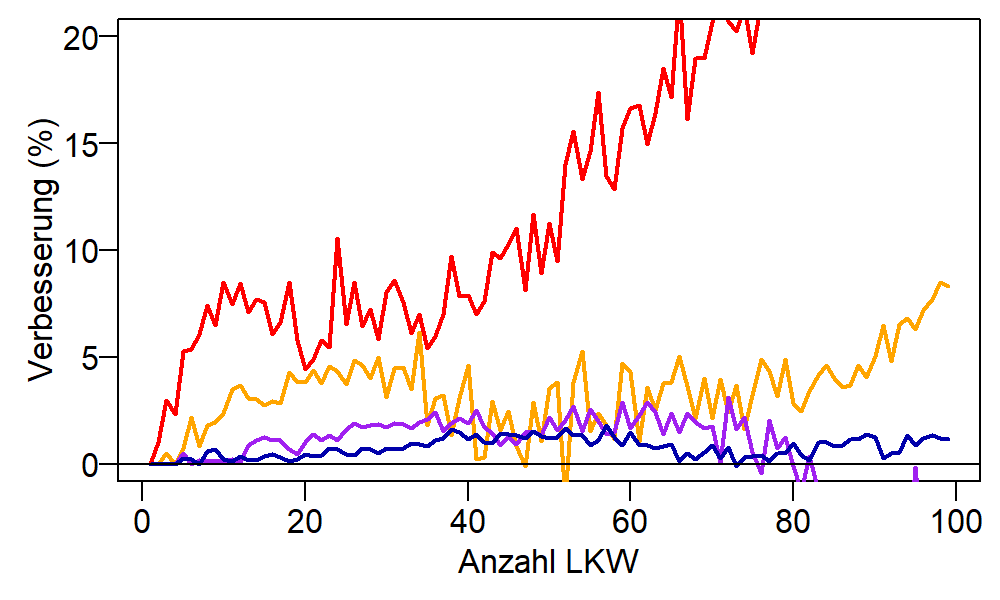
\includegraphics[width=\linewidth]{images/graphs/rsSlotsizeSjn.png}
  \caption{Shortest Job Next}
  \label{fig:eof1}
\end{subfigure}
\begin{subfigure}{.495\textwidth}
  \centering
  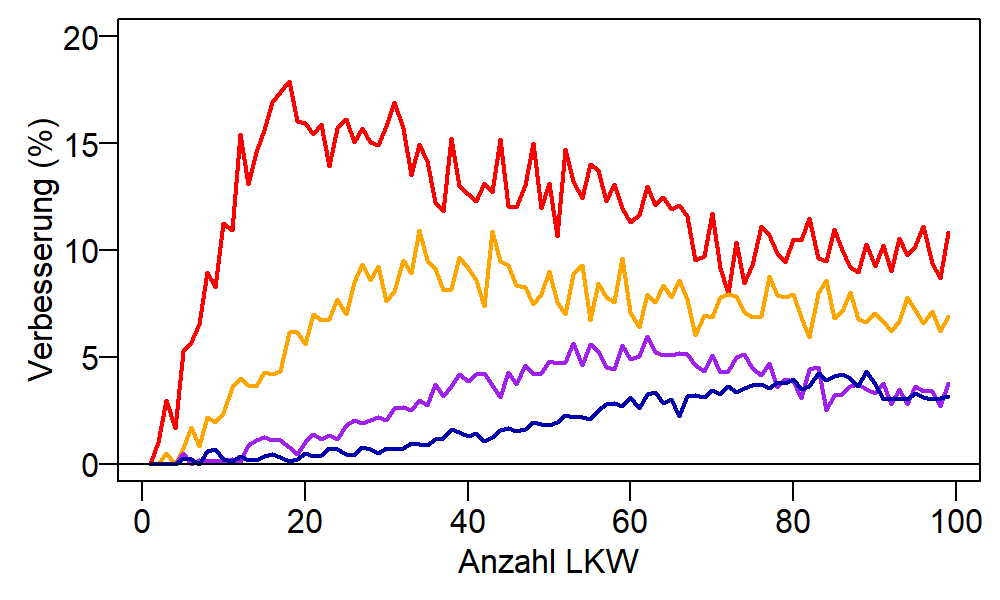
\includegraphics[width=\linewidth]{images/graphs/rsSlotsizeMit.png}
  \caption{Most Idle Time}
  \label{fig:eof2}
\end{subfigure}

\begin{subfigure}{.5\textwidth}
  \centering
  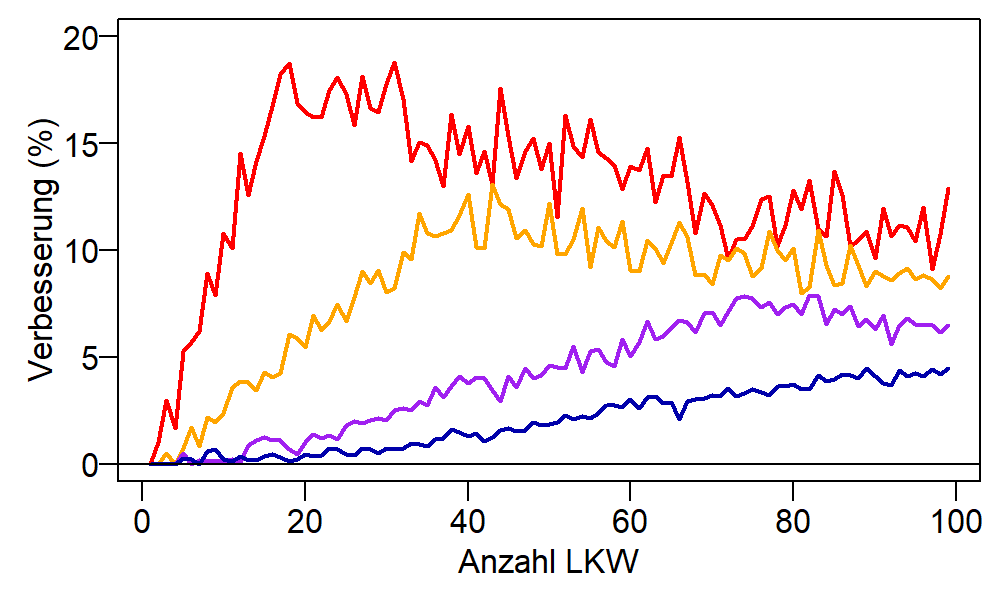
\includegraphics[width=\linewidth]{images/graphs/rsSlotsizeFcfs.png}
  \caption{First come, first served}
  \label{fig:eof3}
\end{subfigure}
\caption{Verbesserung der geplanten LKW bei veränderter Slotgröße}
\label{fig:evalSlotsize}
\end{figure}
\todo{Zuklein?, Legende?!, evtl. auch nicht Verbesserung sondern oScheduled zeigen, wegen streuung?!}

\begin{figure}[H]
\centering
\begin{subfigure}{.495\textwidth}
  \centering
  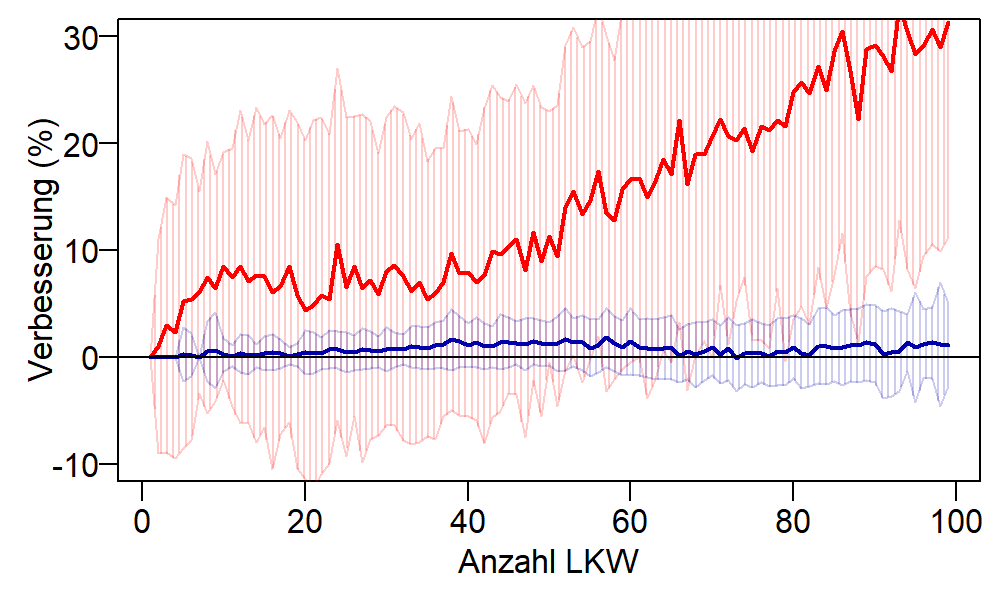
\includegraphics[width=\linewidth]{images/graphs/rsSlotsizeSjn_Streuung.png}
  \caption{Shortest Job Next}
  \label{fig:eofs1}
\end{subfigure}
\begin{subfigure}{.495\textwidth}
  \centering
  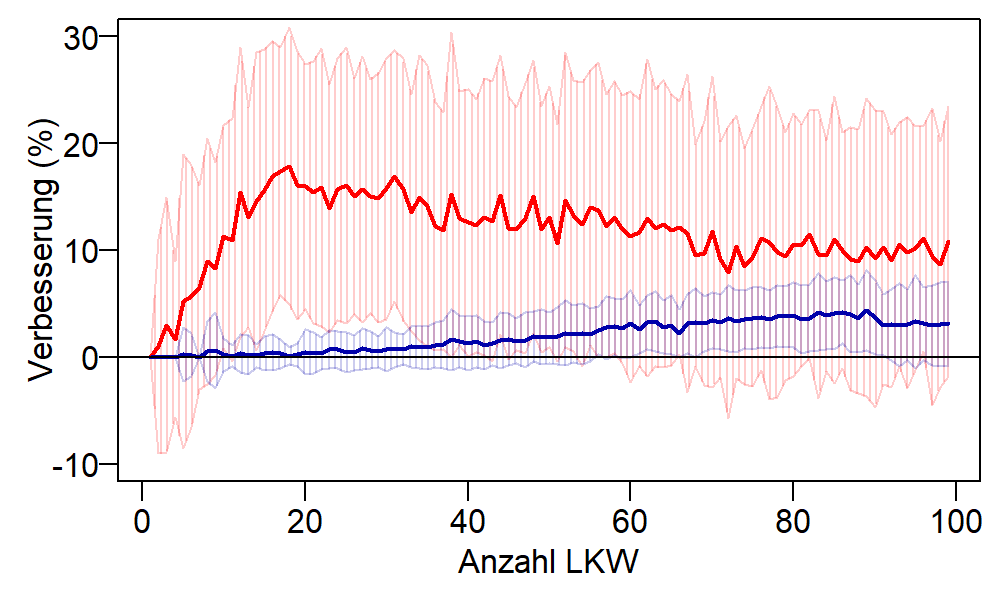
\includegraphics[width=\linewidth]{images/graphs/rsSlotsizeMit_Streuung.png}
  \caption{Most Idle Time}
  \label{fig:eofs2}
\end{subfigure}

\begin{subfigure}{.5\textwidth}
  \centering
  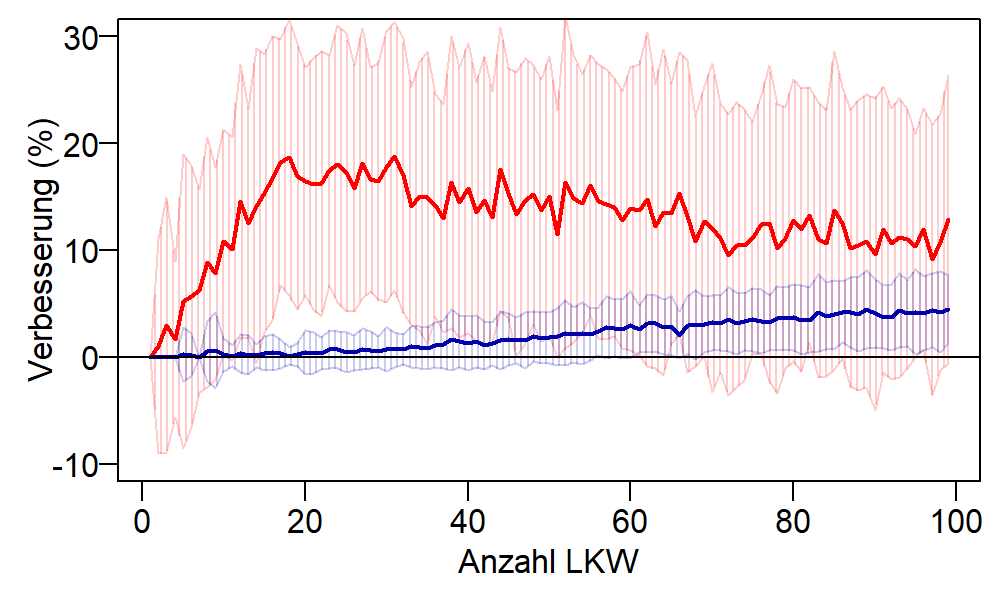
\includegraphics[width=\linewidth]{images/graphs/rsSlotsizeFcfs_Streuung.png}
  \caption{First come, first served}
  \label{fig:eofs3}
\end{subfigure}
\caption{Streuung der Verbesserung der geplanten LKW bei veränderter Slotgröße}
\label{fig:evalSlotsizeStreuung}
\end{figure}
\todo{Zuklein?, Legende?!}

Eine Betrachtung der Testergebnisse (siehe Abb. \ref{fig:evalSlotsize}) zeigt hier tatsächlich unerwartet große Unterschiede auf. In der Gesamtsicht lässt sich schon auf den ersten Blick fetsthalten, dass eine Veränderung der Slotgröße erheblichen Einfluss auf die Verbesserungsrate hat. 

Der Eindruck, dass das SJN Verfahren eher keine allzu guten Ergebnisse liefert, setzt sich hier fort. Die Streuung der Werte ist sehr hoch, insbesondere bei kleinen Slots (siehe Graphen \ref{fig:evalSlotsizeStreuung}). Bei 60 Minuten Slotgröße ist noch eine relativ hohe Verbesserung zwischen 5 und 10\% zu erkennen, welche ab ca. 40 LKW auch noch einmal extrem weiter ansteigt. Je größer die Slots allerdings werden, desto geringer oder sogar negativer wird die Verbesserung. Man könnte nun sagen, dass die Verbesserung beim 60 Minuten Slot wirklich gut ist. Allerdings wurde in den vorherigen Szenarien bereits festgestellt, dass sich eine Überbuchung insgesamt sehr negativ auswirkt. Der extreme Anstieg der Verbesserung kann also gar nicht genutzt werden, da nur die ersten 10-15 LKW wirklich sinnvoll eingeplant werden können. Alle weitere Verbesserung ist nicht nutzbar, da so extrem viele LKW auf andere Slots verschoben werden müssten und sind dann dort sehr negativ auswirken. Auch die hohe Streuung der Werte sprich nicht gerade für ein gutes Verfahren, da kaum konstant positive Ergebnisse erzeugt werden.

Anders sieht es dagegen wieder bei den beiden anderen Verfahren aus. Auch hier lassen sich wieder große Ähnlichkeiten zwischen den Auswertungen der beiden Verfahren feststellen. In allen Kurven ist ein starker Anstieg bis zu einem Maximum zu erkennen und ein anschließender, leichterer Abfall der Verbesserung. Diese Spitze verschiebt sich mit steigender Größe der Slots nach hinten, was auf die größere Kapazität für LKW zurückzuführen ist. Sehr auffällig ist, dass es bei kleineren Slots deutlich höheres Verbesserungspotenzial gibt. Im 60 Minuten Slot erreicht das MIT Verfahren im Durchschnitt bis zu ca. 17\% Verbesserung und das FCFS Verfahren sogar noch mit durchschnittlich etwa 18\% in der Spitze sogar noch etwas mehr. Im 120 Minuten Slot sind es nur noch maximal etwa 11 respektive 13\% in der Spitze. In den weiteren Schritten ist die Abnahme nicht mehr ganz so hoch, aber immer noch sichtbar. Allerdings ist auch in diesen beiden Verfahren die Streuung, gerade bei kleinen Slots sehr hoch (siehe Graphen \ref{fig:eofs2} und \ref{fig:eofs3}).

Schlussfolgernd aus diesem Test lässt sich sagen, dass bei Nutzung der Verfahren MIT oder FCFS durchaus eine kleinere Slotgröße empfehlenswert ist. Was tatsächlich ein sehr spannendes Ergebnis ist. Durch die extreme Streuung gibt es hier durchaus Potenzial für große Verbesserungen, allerdings sind auch sehr geringe Unterschiede zum unoptimierten Fall möglich. In vorherigen Betrachtungen hätte man durchaus zu der Vermutung kommen können, dass größere Slots durch die größere Anzahl von möglichen LKW und somit größeren Planungsspielraum, ein größeres Optimierungspotenzial und somit bessere Ergebnisse liefern. Es ist allerdings auch zu bemerken, dass die Planungsalgorithmen mit steigender Größe der Slots nicht unbedingt schlechter bzw. weniger gut werden. Ein großer Faktor dürfte hier auch sein, dass das bisherige, unoptimierte Verfahren für kleine Slots sehr ungeeignet ist\todo{Das nochmal irgendwo zeigen/belegen?}. Gerade bei kleinen Slots ist eine zufällige Ankunftszeit innerhalb des Zeitraums sehr problematisch, da vor allem am Anfang sehr viele Leerlaufzeiten entstehen, welche sich erst sehr viel später ausgleichen können, wenn mehr LKW warten. Bei kleinen Slots würden dann sehr viel schneller LKW aus dem Zeitfenster herausfallen. Dies führt bei größer werdenden Slots natürlich zu sehr viel mehr abgefertigten LKW und einer besseren Auslastung, die Wartezeiten werden dann aber natürlich hoch sein. Diese hohe Variabilität und der kleine Spielraum bei der Planung führt eben zu dieser hohen Streuung der Werte.


\subsubsection{Testszenario 4: Verhalten bei ungleicher Verteilung benötigter Ressourcen}

Der letzte Eingangsparameter, welcher das Optimierungsergebnis stark beeinflussen dürfte, ist die Art und Anzahl der verfügbaren Ressourcen, bzw. die Verteilung der Art der Ladungen und somit der Bedarf an Ressourcen. Bisher wurde hier immer mit einer ausgeglichenen Verteilung der Ladungsarten gearbeitet und auch die Art und Anzahl der verfügbaren Ressourcen war relativ gut an diesen Fall angepasst. Die Frage die sich nun stellt ist, wie sich die Algorithmen und Optimierungsergebnisse verhalten, wenn hier eine starke Ungleichverteilung herrscht, d.h. wenn sehr viele Ladungen des gleichen Typs ankommen, dann aber keine dazu passende Anzahl von Ressourcen und Ladehilfsmitteln bereitsteht. 

Zu diesem Zweck wurden in diesem Fall die verfügbaren Ressourcen so gelassen, wie sie zuvor auch verwendet wurden, allerdings wurde nun die Anzahl der Buchungen der Kategorie LIFT\_CHAINS schrittweise im Verhältnis zu den übrigen Kategorien erhöht. Die Wertetabellen wurden hier mit der Testklasse \textit{CategoryDistributionTest} erzeugt und mittels des R-Skripts \textit{rsCategoryDistribution.R} \todo{Pfad, etc} ausgewertet. Jeweils dargestellt werden die Ergebnisse für eine Gleichverteilung von 1:1:1:1 und die Verteilungen 3:1:1:1 bzw. 5:1:1:1. Auch hier wurde wieder mit der absoluten Zahl der verplanten LKW gearbeitet, da so die Streuung im unoptimierten Zustand keinen zu großen Einfluss auf die optimierten Werte hat. Jeweils zu erkennen sind die optimerten Werte in der kräftigeren Farbe und zum Vergleich die unoptimerten Durchschnitte in einer etwas helleren Farbe.


\begin{figure}[H]
\centering
\begin{subfigure}{.495\textwidth}
  \centering
  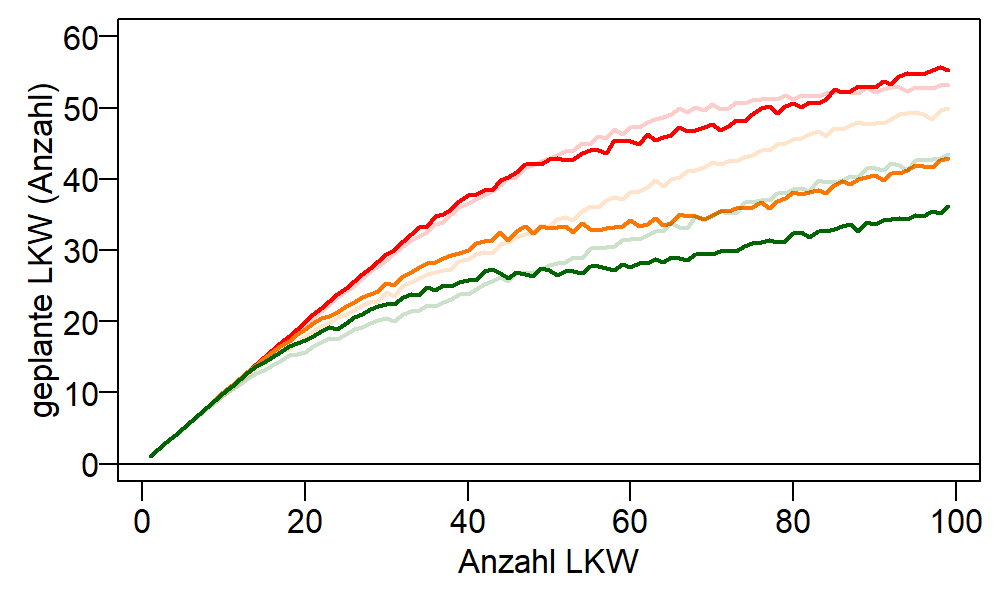
\includegraphics[width=\linewidth]{images/graphs/rsCategoryDistributionSjn.png}
  \caption{Shortest Job Next}
  \label{fig:ecd1}
\end{subfigure}
\begin{subfigure}{.495\textwidth}
  \centering
  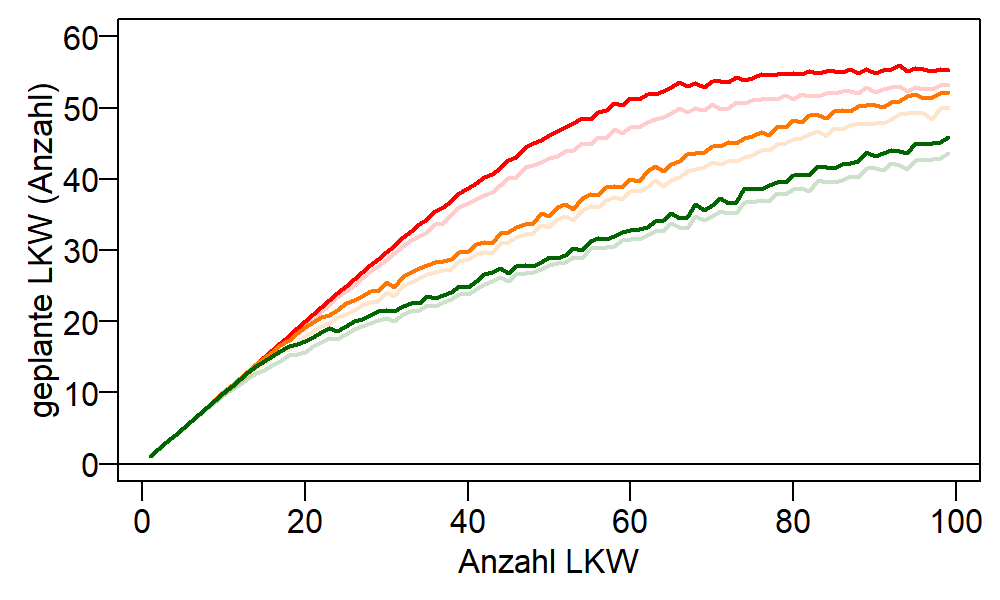
\includegraphics[width=\linewidth]{images/graphs/rsCategoryDistributionMit.png}
  \caption{Most Idle Time}
  \label{fig:ecd2}
\end{subfigure}

\begin{subfigure}{.5\textwidth}
  \centering
  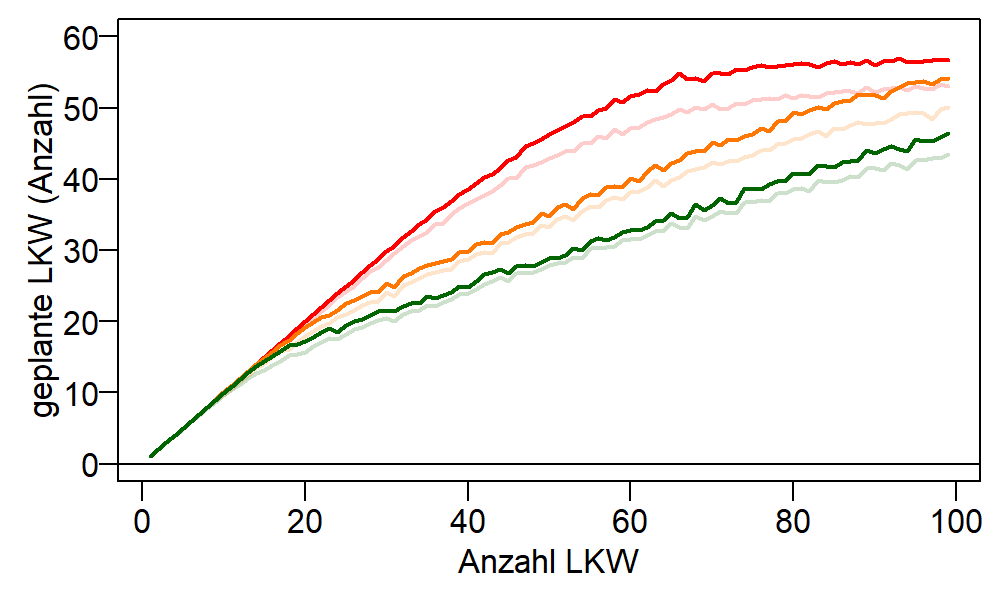
\includegraphics[width=\linewidth]{images/graphs/rsCategoryDistributionFcfs.png}
  \caption{First come, first served}
  \label{fig:ecd3}
\end{subfigure}
\caption{Geplante LKW bei steigender Ungleichverteilung der Abfertigungskategorien}
\label{fig:evalCategoryDist}
\end{figure}
\todo{Legende}

Auch dieses letzte Testszenario verfestigt das Bild und die Bewertung, welche schon zuvor über die einzelnen Verfahren gewonnen wurde. 

Das SJN Verfahren (siehe Graph \ref{fig:ecd1}) zeigt wie auch schon zuvor festgestellt wenig Verbesserung und sogar eine teilweise Verschlechterung der Anzahl der abgefertigten LKW. Extremer wird dieses Verhalten sogar, bei der hier gezeigten Ungleichverteilung. Gegenüber der ausgeglichenen Verteilung ergibt sich hier zunächst ein starker negativer Sprung, aber auch gegenüber der jeweils unoptimierten Kurve sind hier starke Verschlechterungen erkennbar. Je ungleicher die Verteilung wird, das Ergebnis aber nicht mehr ganz so viel schlechter. Es ist allerdings auch zu erkennen, dass die Verbesserung gegenüber dem unoptimierten Fall im unteren Bereich zwischen etwa 20 und 40 LKW leicht steigt, wenn die Verteilung unausgeglichener ist. Insgesamt war dieses Verfahren aber ohnehin schon kein Favorit für einen realen Einsatz, spätestens aber wenn keine gute Prognose der Verteilung der ankommenden LKW möglich ist und somit keine dazu passenden Ressourcen zur Verfügung gestellt werden können, verschlechtert sich die Performance stark.

Die Verfahren MIT und FCFS, verhalten sich hier wie auch schon in den vorherigen Auswertungen sehr ähnlich, wie Graphen \ref{fig:ecd1} und \ref{fig:ecd2} zeigen. Auch hier hat FCFS mit höherer Zahl von LKW wieder leicht höhere Werte als MIT. Erkennbar ist, dass die Anzahl der erfolgreich eingeplanten LKW deutlich sinkt, wenn es eine stärkere Ungleichverteilung gibt. Gleichzeitig nimmt auch die Verbesserung gegenüber dem unoptimerten Fall ab. Im für einen 180 Minuten Slot interessanten Fall bis ca. 60 LKW erreicht der Unterschied der Kurven sein Maximum. Dass sich der Nachteil dieser Verteilung mit noch weiter steigender Zahl wieder verringert, ist also in der Realität weniger relevant. Es lässt sich daraus schließen, wie auch schon zu erwarten war, dass es schon im vorhinein das Ziel sein sollte, eine möglichst gute Prognose der ankommenden LKW zu haben, zumindest was die Verteilung der Ladungstypen angeht. Wenn einfach keine passenden Aufträge für die zur Verfügung stehenden Maschinen hereinkommen, kann auch der beste Algorithmus keine gute Auslastung aller Ressourcen erzeugen. Dennoch erkennt man, dass beide Algorithmen weiterhin eine verbesserte Verteilung und somit die Planung von mehr LKW ermöglichen, auch wenn dieser Vorteil natürlich geringer wird.


\subsection{Auswertung Algorithmus 2 (TSP)}

Die Kernpunkte der Auswertung des zweiten Algorithmus unterscheiden sich etwas von den Zielen der anderen Auswertung. Zum einen soll hier auch wieder eine Bewertung hinsichtlich der Art und Höhe der möglichen Optimierungen stattfinden. Im Unterschied zur anderen Umsetzung sollen die Lösungsverfahren des TSP theoretisch die gleiche, beste Lösung ermitteln. Ein erstes Ziel wäre es also alle Verfahren bezüglich ihrer Nutzbarkeit und Praxisuntauglichkeit zu bewerten, um alle anschließenden Tests dann nur mit dem daraus bestimmten, besten Verfahren durchzuführen.

\subsubsection{Testszenario 1: Bestimmung der Parameter für das Simulated Annealing Verfahren}

Bevor die Verfahren gegeneinander bewertet werden können, müssen zunächst einmal die besten Werte für das Simulated Annealing Verfahren gefunden werden. Die variablen Paramater sind dabei: startingTemperature, coolingRate und numberOfIterations. Ziel dieses Testszenarions ist es, diese Parameter zu variieren und so die bestmöglichen Eingabewerte für den gegebenen Anwendungsfall zu finden. In der Testklasse \textit{SimAParameterTest} wurden dafür die im Folgenden beschriebenen Abläufe implementiert, mit dem R-Skript \textit{tspSimAParameter} wurden die Ergebnisse ausgewertet, sowie die hier dargestellten Graphen erzeugt.

Schaut man sich die Implementierung des Algorithmus genauer an, so ist numberOfIterations einfach die maximale Anzahl von Schleifendurchläufen und sozusagen eine Begrenzung, damit der Algorithmus im schlimmsten Fall nicht ewig läuft. Um diesen Parameter sinnvoll einschätzen zu können, wurden alle folgenden Testdurchläufe mit dem Wert Integer.MAX\_VALUE durchgeführt, somit wird es so viele Schleifendurchläufe geben, wie es braucht. Die benötigte Anzahl wird hier jeweils in die CSV-Datei mit den Ergebnisdatensätzen übernommen. Somit können hier im Nachhinein die höchsten benötigten Werte abgelesen werden, um eine sinnvolle Einschätzung der notwendigen Iterationen zu erhalten und für den Worst-Case ein mit Spielraum versehenes Limit gesetzt werden. Hauptsächlich abhängig ist das Ergebnis des Algorithmus also von startingTemperature und coolingRate. Die startingTemperature darf sich dabei in einem theoretischen Bereich von >0,1 und unendlich bewegen. Die coolingRate muss für sinnvolle Ergebnisse >0 und <1 sein. Um hier einen Gesamteindruck der Auswirkung dieser beiden Parameter auf das Ergebnis zu erhalten, sollen diese beiden Variablen systematisch in Schleifen variiert werden und jeweils die Kosten berechnet werden. Es entsteht somit ein dreidimensionaler Datensatz der Kosten in Abhängigkeit von startingTemperature und coolingRate. Für das Gesamtbild wird ein zufälliger, aber fester Graph generiert. Mit diesem wird der SimA Algorithmus mit jeder Kombination von startingTemperature und coolingRate einmal ausgeführt. Um das Verhalten über verschiedenen Graphen zeigen zu können, wird dieser gesamte Prozess mit 100 verschiedenen Graphen ausgeführt. In ersten, losen Test hat sich gezeigt, dass der wirklich interessante Teil bei startingTemperature etwa im Intervall [1;100] liegt und die coolingRate etwa bei [0.9;1[. Um die Übersichtlichkeit zu wahren und die Ausführungsdauer der Tests einzuschränken, wurden die Tests deshalb auf diese Intervalle konzentriert. Die startingTemperature wurde dabei in Schritten von 1 erhöht, die coolingRate jeweils um 0,001.

Nachfolgende Graphen (Abb. \ref{fig:evalSimAParams}) zeigen das Ergebnis dieser Auswertung. Gezeigt werden dabei in einem farblichen Verlauf die durchschnittlichen Kosten über aus den 100 Durchläufen mit verschiedenen Graphen zu einem Paar aus startingTemperature und coolingRate. Die grünen Bereiche zeigen dabei, wo die Kosten tendenziell am geringsten sind und die roten Bereiche repräsentieren die höchsten Kosten. Da auch die Größe des zu bearbeitenden Graphen einen Einfluss hat, wurde dieser gesamte Test mit Graphen mit den Größen 10, 20, 50 und 100 Knoten wiederholt. Mit Blick auf die zu erwartenden LKW \todo{in konzeption/Anforderungen erwähnen?!} wird dies wird voraussichtlich der Bereich sein, in dem der Algorithmus zum Lösen des TSP verwendet wird.

\begin{figure}[H]
\centering
\begin{subfigure}{.495\textwidth}
  \centering
  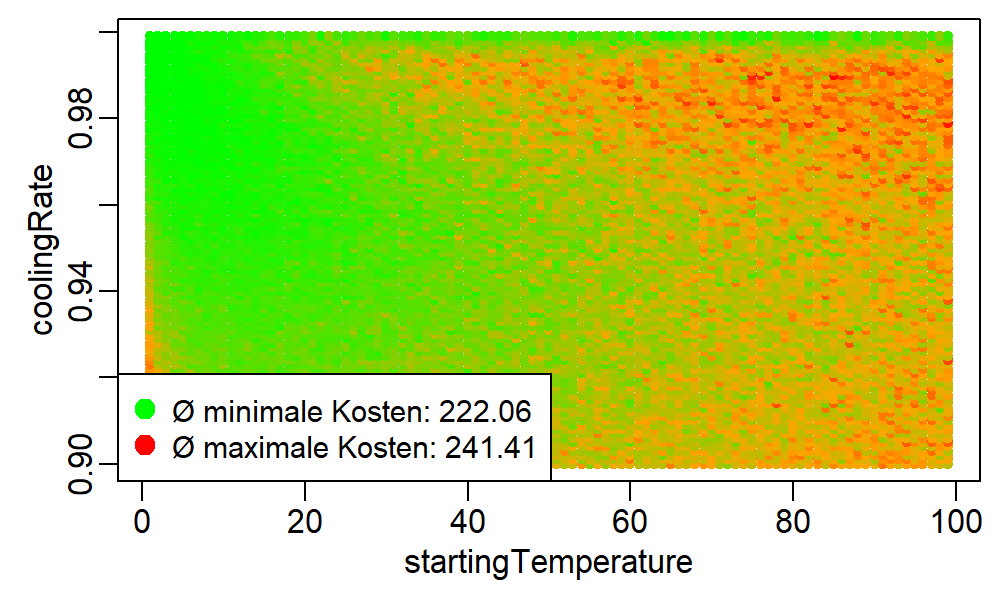
\includegraphics[width=\linewidth]{images/graphs/tspSimAParameter10.png}
  \caption{Graph mit 10 Knoten}
  \label{fig:esp1}
\end{subfigure}
\begin{subfigure}{.495\textwidth}
  \centering
  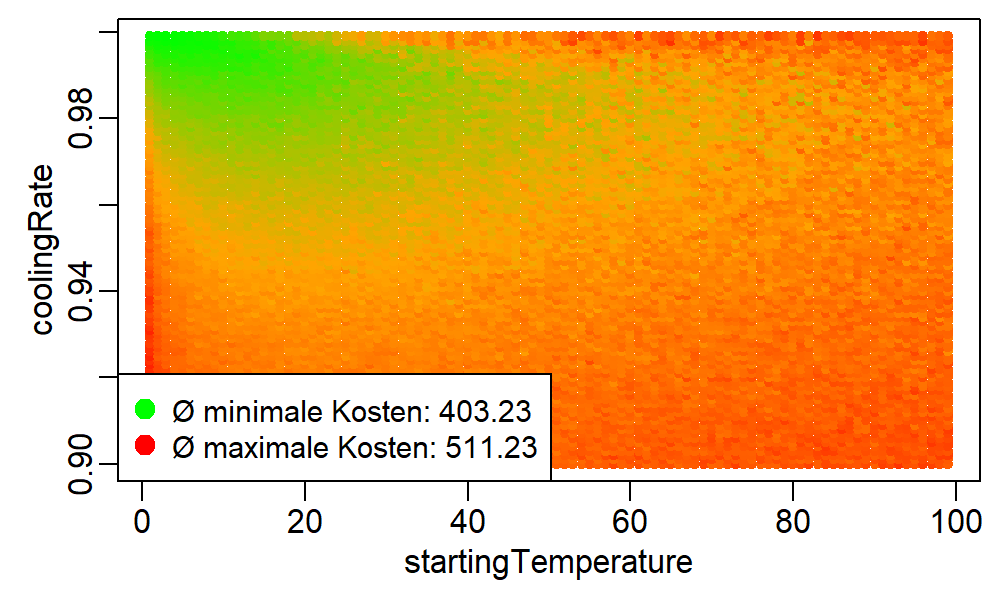
\includegraphics[width=\linewidth]{images/graphs/tspSimAParameter20.png}
  \caption{Graph mit 20 Knoten}
  \label{fig:esp2}
\end{subfigure}

\begin{subfigure}{.495\textwidth}
  \centering
  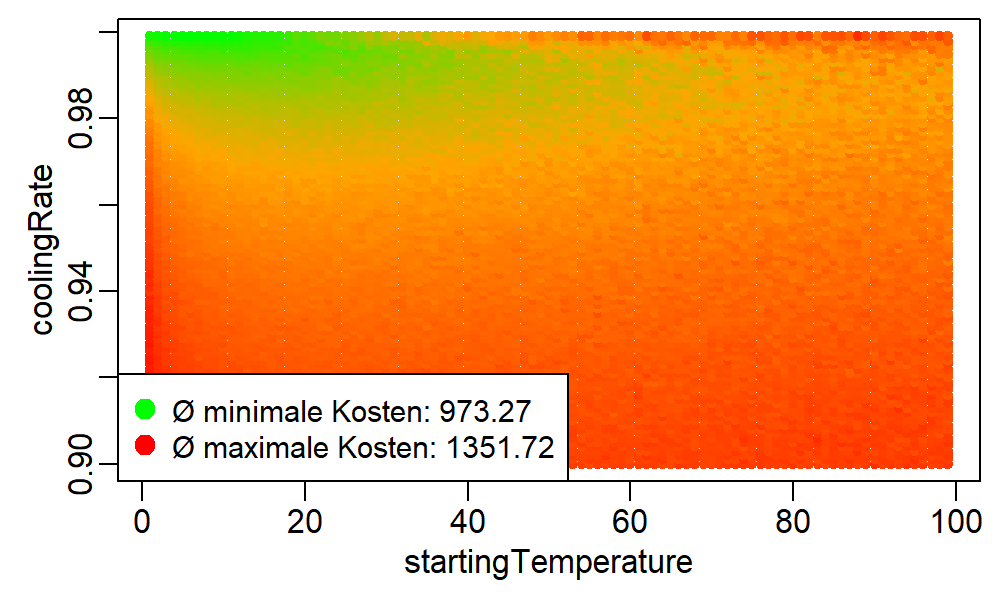
\includegraphics[width=\linewidth]{images/graphs/tspSimAParameter50.png}
  \caption{Graph mit 50 Knoten}
  \label{fig:esp3}
\end{subfigure}
\begin{subfigure}{.495\textwidth}
  \centering
  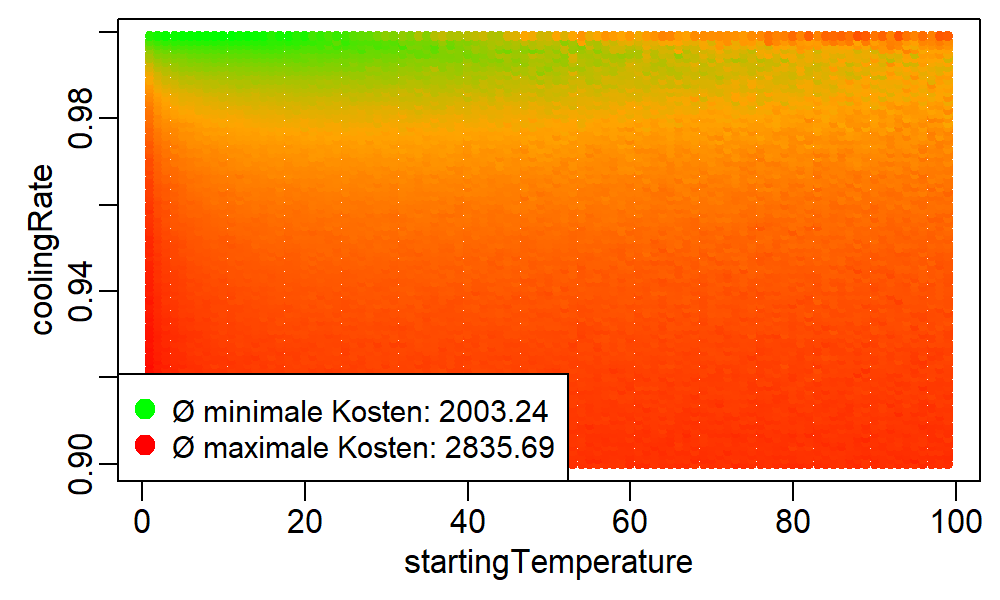
\includegraphics[width=\linewidth]{images/graphs/tspSimAParameter100.png}
  \caption{Graph mit 100 Knoten}
  \label{fig:esp4}
\end{subfigure}
\caption{Simualted Annealing mit variierten Parametern}
\label{fig:evalSimAParams}
\end{figure}

Für die besten Werte der Parameter lassen sich daraus nun einige Schlussfolgerungen ziehen. Zur benötigten Anzahl von Iterationen lässt sich aus den resultierenden Wertetabellen ablesen, dass diese relativ stark schwankt, das Maximum liegt in diesem Beispiel aber bei 6895\todo{finalen Wert eintragen}. Selbst wenn man die Grenze für den Worst-Case nun extrem großzügig auf beispielsweise 100.000 setzt, ist dies immer noch ein Wert, der in der Berechnung problemlos handhabbar ist. Selbst diese Zahl von Iterationen sollte nicht für nennenswert hohe Ausführungszeiten sorgen. Diese Höhe von Iterationen wird aber wenn überhaupt ohnehin extrem selten erreicht.

Die dargestellten Graphen lassen nun eine gute Einschätzung zu, wie die beiden weiteren Parameter zu wählen sind. Grundsätzlich werden sich dabei keine exakten Werte bestimmen lassen, da es sich hier immer noch um Zufallswerte handelt, für die immer etwas andere Parameter optimal wären. Gerade bei geringer Anzahl von Knoten ist zu erkennen, dass die Kosten auch bei nah aneinander liegenden Punkten deutliche Schwankungen haben, da sehr unterschiedlich farbige Punkte nah beieinander liegen und kein gleichmäßiger Verlauf entsteht. Dennoch lässt sich eine sehr gute Tendenz erkennen, bei welcher Kombination von Parametern die Kosten optimal gering werden. Bei geringer Anzahl von Knoten ist die Wahl der Parameter noch nicht ganz so kritisch, hier ist der optimale, grüne Bereich noch relativ groß. Hier würde eine startingTemperature $<$ 50 und eine coolingRate $>$ 0,9 in der Regel schon sehr gute Werte liefern. Mit größerer Anzahl von Knoten wird dieser Bereich deutlich kleiner. Hier sollte vor allem die coolingRate so nah wie möglich an 1 liegen. Gute Werte werden hier tendenziell nur noch bei startingTemperature $<$ 40 und coolingRate $>$ 0,99 erzielt. Die grünen Bereiche der Graphen überschneiden sich allerdings, was sehr gut es, denn gut Werte für 100 Knoten liefern somit auch z.B. bei 10 Knoten ebenfalls gute Ergebnisse. Eine startingTemperature von 15 und eine coolingRate von 0,9995 sollten also gut geeignet sein.

Abschließend wurden die hier ermittelten Werte (numberOfIterations=100.000, startingTemperature=15, coolingRate=0,9995) als Standardwerte in die Variablen der Klasse \textit{SimulatedAnnealingAlgorithm} übernommen. Über in diesen Tests verwendeten Konstruktor können wie bisher variable Werte verwendet werden, werden diese Werte allerdings über den weiteren Konstruktor nicht gesetzt, so werden immer die hier ermittelten, besten Werte verwendet. Alle weiteren Testszenarien arbeiten also dann direkt mit diesen Werten.

\subsubsection{Testszenario 2: Laufzeit und Grenzen}
\todo{Leistungsdaten des Rechners angeben?!}

Wie schon bei der Implementierung aufgefallen ist, werden insbesondere die exakten Verfahren früher oder später durch ihre Laufzeit bei der Berechnung oder durch ihren Arbeitsspeicherbedarf begrenzt sein. Der nötige Aufwand ist dabei zum bedeutendsten Teil von der Anzahl der Knoten des zu lösenden Graphen abhängig. Um also zunächst die Lösungsverfahren selbst zu bewerten, sind hier noch gar keine Vergleiche und Auswertungen hinsichtlich des eigentlichen Problemszenarios nötig. Viel mehr ist hier die Laufzeit bei der Berechnung der Ergebnisse für die einzelnen Verfahren von Interesse. Aus diesem Grund arbeiten die folgenden Tests, welche in der Testklasse \textit{RunTimeTest} implementiert wurden auch direkt mit den Algorithmus-Klassen, ohne Ladeplätze, Slotlimiterungen o.ä. zu berücksichtigen. Ausgeführt wird also immer jeder Algorithmus einmal mit dem identischen Eingangsgraphen. Dabei wird schrittweise die Anzahl der Knoten erhöht. Für jede Anzahl von Knoten werden dabei 10 Durchläufe mit unterschiedlichen, zufälligen Graphen erzeugt, um sinnvolle Durchschnittswerte und Streuungen bei der Berechnungszeit ermitteln zu können. Da hier keine exakten Ergebnisse, sondern vor allem Größenordnungen interessant sind, reichen hier 10 Wiederholungen. Um die Ausführungszeit darüber hinaus im Rahmen zu halten, wurde ein Begrenzung eingebaut, sodass die Algorithmen für mehr Knoten nicht mehr ausgeführt werden, wenn entweder einmal der Speicherplatz ausgegangen ist oder wenn die Ausführung zu lange gedauert (Limit von 10 Minuten) \todo{Erhöhen für eine Ausführung von 16 Knoten?!} hat. Die Tendenz sollte dann erkennbar sein und eine stunden- oder tagelange Ausführung der Tests ist nicht nötig. Die folgende Auswertung (Tabelle \ref{tab:evalTspRunTime}) wurde durch das R-Skript \textit{tspRunTime.R} berechnet. Als Darstellungsform wurde in diesem Fall eine Tabelle gewählt, da sich die Werte stark voneinander unterscheiden. Die wichtigen Aspekte wären in einem Graphen nicht gut sichtbar.


\begin{table}[H]
    \caption{Durchschnittliche Laufzeiten der Verfahren (Alle Werte in s)}
    \label{tab:evalTspRunTime}
    \centering
    \begin{tabular}{c|c|c|c|c|c|c}
        \textbf{Knoten} & \textbf{Ø SimA} & \textbf{$\sigma$ SimA} & \textbf{Ø BnB} & \textbf{$\sigma$ BnB} & \textbf{Ø RM} & \textbf{$\sigma$ RM} \\\hline\hline
        \csvreader[
            %column count=4,
            %no head,
            %table head=\hline\hline,
            %table head=\textbf{Labels} & \textbf{Labels} & \textbf{Labels} & \textbf{Labels} \\\hline,
            late after line=\\\hline,
            late after last line=\\
        ]
        {files/tspRunTime_out.csv}
        {1=\one, 2=\two, 3=\three, 4=\four, 5=\five, 6=\six, 7=\seven, 8=\eight}
        {\two & \three & \four & \five & \six & \seven & \eight}
    \end{tabular}
\end{table}
\todo{Mit mehr Durchläufen asuführen, sternchen an einfach ausgeführten einfügen}

Sehr deutlich zu erkennen ist, dass der Aufwand zum Lösen des Problems exponentiell mit der Anzahl der Knoten steigt. Insbesondere für das Reduced Matrix und das Branch and Bound Verfahren bedeutet dies, dass der Aufwand ab etwa 10 Knoten merklich höher wird und jeweils bei 13 bzw. 15 Knoten so groß wird, dass dies zumindest für eine größere Zahl von Wiederholungen in dieser Auswertung deutlich zu viel ist. Das Reduced Matrix Verfahren scheitert dabei an einem \glqq{}java.lang.OutOfMemoryError: Java heap space\grqq{} Fehler, welcher zeigt, dass der Arbeitsspeicher der Java VM nicht ausreicht, selbst mit einer Erhöhung auf 8 GB. Die Laufzeit der Berechnung steigt zwar auch erheblich, aber dem ersten Anschein nach nicht so schnell wie im Branch and Bound Verfahren. Hier kostet bereits die Berechnung von 15 Knoten im Durchschnitt ca. 16 Minuten, während es bei 14 Knoten noch ca. 3 Minuten waren. Aus diesem Grund wurden auch die letzten Durchläufe jeweils nur mit einer Wiederholung durchgeführt und bilden somit nur einen Anhaltspunkt der Ausführungszeit, aber keinen sinnvollen Durchschnitt mehr\todo{finaler Stand?}. Bei diesen Verfahren zeigt sich aber auch eine hohe Standardabweichung bei der Ausführungszeit zwischen verschiedenen Durchläufen. Dies dürfte damit zusammenhängen, dass diese Verfahren je nach Eingabewerten unterschiedlich viel Zeit sparen. Das Simulated Annealing Verfahren zeigt dagegen über wesentlich längere Zeit deutlich geringere Ausführungszeiten. Insgesamt ist bei der mehrfachen Ausführung dieser Testklasse sichtbar geworden, dass die Ausführungszeiten auch zwischen diesen Ausführungen schwanken. Dies hat insbesondere beim Branch and Bound Verfahren mit 14 Knoten einen sichtbaren unterschied von einigen Sekunden gemacht. Dies dürfte auch mit der sonstigen Auslastung des Computers im Hintergrund zu tun haben. Eine deutliche Tendenz ist aber sehr klar sichtbar und ändert nichts an den extrem steigenden Zeiten.




\textbf{Qualität der Verfahren}

Gleichzeitig sind die Werte dieses Szenarios ein guter Anhaltspunkt, um die Qualität der Verfahren untereinander zu vergleichen. Insbesondere das Simulated Annealing Verfahren findet nicht unbedingt das beste Ergebnis, sodass hier auch gleichzeitig ein direkter Vergleich stattfinden kann. Als Metrik bietet sich hier die Höhe der Gesamtkosten bzw. der Gesamtzeit des gefundenen Weges durch den Graphen an, da dies auch der Wert ist, nachdem beim TSP optimiert wird. Diese zweite Auswertung (siehe Tabelle \ref{tab:evalTspTotalCost}) wurde mit den identischen CSV-Daten durch das R-Skript \textit{tspTotalCost.R} berechnet. Auch hier wurde die Darstellung in einer Tabelle gewählt, da übereinanderliegende und starkt steigende Werte so deutlich besser sichtbar sind.

\begin{table}[H]
    \caption{Durchschnittliche Kosten der Verfahren (Alle Werte in min)}
    \label{tab:evalTspTotalCost}
    \centering
    \begin{tabular}{c|c|c|c|c|c|c}
        \textbf{Knoten} & \textbf{Ø SimA} & \textbf{$\sigma$ SimA} & \textbf{Ø BnB} & \textbf{$\sigma$ BnB} & \textbf{Ø RM} & \textbf{$\sigma$ RM} \\\hline\hline
        \csvreader[
            late after line=\\\hline,
            late after last line=\\
        ]
        {files/tspRunTime_costOut.csv}
        {1=\one, 2=\two, 3=\three, 4=\four, 5=\five, 6=\six, 7=\seven, 8=\eight}
        {\two & \three & \four & \five & \six & \seven & \eight}
    \end{tabular}
\end{table}
\todo{Mit mehr Durchläufen ausführen, sternchen an einfach ausgeführten einfügen}

\todo{Streuung sinnvoll, da immer andere Graphen?! Oder hier evtl Variationskoeffizient, um relative schwankung darzustellen?}

Erkennbar ist, die exakten Verfahren BnB und RM durchgängig identische Werte liefern. Die Abweichung von RM bei 13 Knoten ist damit zu erklären, dass hier aufgrund vom Speichermangel nicht mehr alle Durchläufe berechnet werden konnten, während es bei BnB ein Durchschnitt aus allen 10 Iterationen ist. Auch das SimA Verfahren zeigt bis 10 Knoten identische Werte. Dies zeigt, dass in diesen Bereichen von allen Verfahren das gleiche und serh wahrscheinlich auch optimale Ergebnis erzielt wurde. Ab 11 Knoten fängt es an, dass die Ergebnisse des SimA Verfahrens etwas schlechter werden, als die höchst wahrscheinlich optimalen Ergebnisse der anderen Verfahren. Aufgrund der bereits erkannten Beschränkungen bezüglich Laufzeit und Speicherbedarf lässt sich diese Tendenz so einfach nicht weiter bestätigen. Dies bestätigt aber auch die Theorie des Simulated Annealing, dass eben in der Regel ein sehr gutes, aber nicht perfektes Ergebnis erzielt wird \todo{Quelle?}. Somit lässt sich vermuten, dass die Ergebnisse auch bei einer sehr viel größeren Zahl von Knoten sehr gut sind.

Insgesamt zeigt sich als großer Vorteil des Simulated Annealing Verfahrens, dass schon mit einfachen Rechen-Ressourcen eine wesentlich höhere Zahl von Knoten, weit über 1000 Knoten möglich ist. Dies übersteigt die hier realistisch zu erwartende Größe von Graphen um ein vielfaches. Insbesondere wenn ein mTSP, also eine Verteilung für mehrere Ladeplätze ermittelt werden soll und somit noch einige Knoten für Ladeplätze verbraucht werden, sind 12-15 Knoten sehr schnell erreicht. Ein sinnvoller Einsatz von Branch and Bound und Reduced Matrix Verfahren ist (in der hier implementierten Variante) also eigentlich nicht möglich. Selbst wenn man die Rechen-Ressourcen deutlich aufstockt, wird der Bedarf weiter exponentiell steigen. Damit ist möglicherweise eine Erhöhung der Knotenanzahl im unteren einstelligen Bereich möglich, eine sinnvoll nutzbare Anzahl wird dies aber höchstwahrscheinlich immer noch nicht. Für die weiteren Tests wird deshalb mit dem Simulated Annealing Verfahren weiter gearbeitet.


\subsubsection{Testszenario 3: Streuung zwischen den Simulated Annealing Durchläufen}

In diesem Szenario geht es darum, wie groß die Streuung der optimierten Kosten beim mehreren Durchläufen des selben Graphen ist. Während vorherigem explorativen Ausprobierens der Verfahren ist aufgefallen, dass sich die Ergebnisse, also die Gesamtkosten zwischen den Durchläufen eines eigentlich identischen Graphen unterscheiden. Dies dürfte aber nur für den Simulated Annealing Ansatz relevant sein, da hier mit gewissen Zufallsprozessen, dem \glqq{}Abkühlungsvorgang\grqq{} gearbeitet wird. Bei den anderen Verfahren ergibt sich immer das beste Ergebnis, bei allerdings höherer Rechenzeit, wie die vorherigen Tests gezeigt haben. Da mit dem Simulated Annealing Verfahren weiter gearbeitet werden soll, soll dieser Umstand an dieser Stelle aber noch einmal genauer untersucht werden.

Das Vorgehen, welches in der Testmethode \textit{spreadTest()} der Testklasse \textit{SimulatedAnnealingTest} implementiert wurde und zur Ermittlung passender Werte dient, ist wie folgt: Die prinzipielle Idee ist es, das Simulated Annealing Verfahren mit dem identischen Eingangsgraphen mehrfach laufen zu lassen. Es wird dabei bei jeden weiteren Durchlauf immer das beste Ergebnis, also die geringsten Durchlaufkosten aller vorherigen Iterationen gespeichert. Die Idee dabei ist, dass man angesichts des geringen Zeitaufwands eines SimA Durchlaufs einfach immer mehrere Durchläufe macht und das insgesamt beste Ergebnis zurück gibt. Um auch hier wieder einen aussagekräftigen Durchschnitt ermitteln zu können, wird das Ganze in einer Schleife mit 100 verschiedenen Graphen durchgeführt. Dargestellt wird immer die prozentuale Abweichung von dem insgesamt für diesen Graphen besten ermittelten Wert, welcher nach Formel \ref{eq:simaResBestCost} berechnet wurde. Diese Darstellung wurde gewählt, da der absolut beste Wert je nach Graphen etwas unterschiedlich ist. In dieser Aufbereitung lässt sich ein besserer Vergleich ziehen. Allerdings ist dieser Wert auch nicht als überhaupt minimal erreichbarer Wert zu verstehen, aber auch bei noch wesentlich mehr Durchläufen bleibt die Kurve nicht konstant bei 0\%, da es sich aber um wenige Fälle und nur noch minimale Verbesserungen handelt, wurde hier der Übersicht halber 70 Durchläufe als Maximum gewählt. Als Größe für den Graphen wurden hier exemplarisch 50 LKW bei 3 Ladeplätzen gewählt, was mit insgesamt 53 Knoten im oberen erwartbaren Bereich liegt, was die potenzielle Größe der Graphen angeht. Je Größer der Graph ist, desto mehr Algorithmus Durchläufe wird es tendenziell benötigen, um das absolut mögliche Minimum zu finden.

\begin{equation} \label{eq:simaResBestCost}
relativ Beste Kosten = \left(\left(\frac{absolut Beste Kosten}{minimale Kosten Der Iteration}\right)*100\right)-100
\end{equation}

\begin{figure}[H]
    \centering
    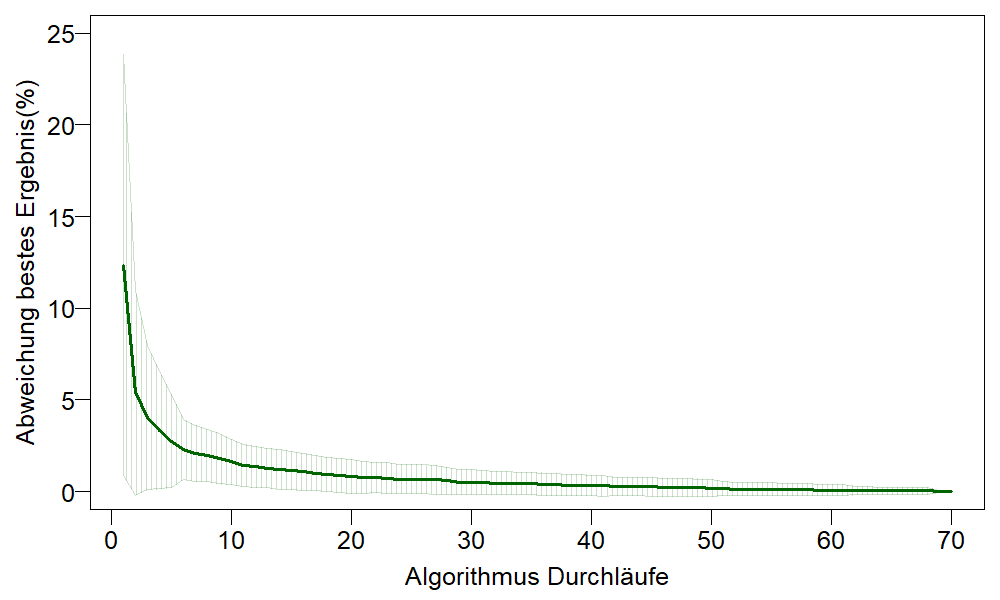
\includegraphics[width=0.7\textwidth]{images/graphs/tspResultSpreadTest.png}
    \caption{Bestes Ergebnis des Simualted Annealing Verfahrens nach mehreren Durchläufen}
    \label{fig:tspEvalSpread}
\end{figure}

\todo{Legende}

In Abbildung \ref{fig:tspEvalSpread} ist erkennbar, dass es zu Beginn mit nur einem einzigen Algorithmuslauf eine sehr große Unsicherheit gibt. Im Durchschnitt ist das Ergebnis etwa 12\% schlechter, als es im besten Fall nach 70 Durchläufen möglich war. Auch die Standardabweichung ist extrem hoch, d.h. es gibt Fälle in denen das Ergebnis nach einem Durchlauf bereits sehr gut ist, in anderen Fällen ist dies da aber noch sehr viel schlechter. Die Kurve sinkt allerdings schon nach wenigen Durchläufen sehr stark. Nach etwa 5 Läufen ist das Ergebnis im Mittel nur noch ca. 3\% schlechter bei auch sehr viel geringerer Streuung. Ab ca. 10 Läufen werden die Ergebnisse auch deutlich langsamer besser.  Für den realen Einsatz des Simulated Annealing Verfahrens lässt sich daraus schlussfolgern, dass eine wiederholte Ausführung zum finden des besten Ergebnisses durchaus sinnvoll ist. Schon eine 5 bis 10-fache Iteration kann die größten Unsicherheiten beseitigen. Angesichts der wirklich sehr geringen Laufzeiten im Millisekunden-Bereich (siehe Tabelle \ref{tab:evalTspRunTime}), kann man sogar über eine wesentlich höhere Zahl von 30 bis 50 oder sogar noch mehr Durchläufen nachdenken. Selbst wenn dann Berechnungszeiten von wenigen Sekunden entstehen, ist dass für den realen Einsatz noch lange kein Problem.


\subsubsection{Testszenario 4: Verbesserung der Abfertigungszeit}

Nachdem nun viel Aufwand in die Bestimmung des besten Lösungsverfahrens sowie in die beste Verwendung der Verfahren geflossen ist, sollen nun Versuche zum eigentlichen Ziel der Optimierung durchgeführt werden. Gearbeitet werden soll dabei, wie in den vorherigen Tests bestimmt wurde, mit dem Simulated Annealing Alogrithmus. Genutzt wird immer das beste Ergebnis aus 50 Durchläufen. Außerdem werden die Buchungen immer auf 3 Ladeplätze aufgeteilt. Interessant ist hier in erster Linie, wie viel sich die gesamte Abfertigungszeit gegenüber dem unoptimierten Ausgangszustand verbessern lässt. Es wird dabei immer die durch den SimA-Algorithmus optimierten Wert mit den unoptimierten Werten verglichen, welche mit aus der Zeitplanung des UnoptimizedAlgorithm ermittelt wurden. Einmal soll das Ganze für einen unbegrenzten Zeitraum simuliert werden. Die gleichen Tests werden aber auch noch einmal für einen begrenzten Slot durchgeführt werden. Interessant sind diese Werte, da dies auch schlussendlich das für den realen Einsatz bedeutende Ergebnis ist. Da die Begrenzung allerdings ein weiterer, auf die eigentliche Optimierung aufbauender Schritt ist, wird hier diese getrennte Betrachtung durchgeführt. Implementiert wurden die Tests in den Testmethoden \textit{test3LoadersBestOf50()} und \textit{test3LoadersBestOf50Limited()} der Testklasse \textit{SimulatedAnnealingTest}. Das R-Skript \textit{tspOptimization.R} diente zur Auswertung.

Im Graphen dargestellt ist zum einen, wie sich die Gesamtzeit verbessert hat, bis alle LKW bearbeitet wurden. Berechnet wurde dieser Wert nach Formel \ref{eq:tspCostSaving}. Zusätzlich ist eine Kurve sichtbar, welche die Verbesserung bei der Zahl der eingeplanten LKW zeigt. Dieser Wert wird über Formel \ref{eq:tspSchedImpr} berechnet. Beide Werte werden prozentual dargestellt, da so ein relativer Vergleich mit steigender Anzahl von LKW Buchungen möglich ist.

\begin{equation} \label{eq:tspSchedImpr}
schedImpr = \dfrac{oScheduledJobs-uScheduledJobs}{uScheduledJobs} * 100
\end{equation}

\begin{equation} \label{eq:tspCostSaving}
costImpr = \dfrac{uCost-oCost}{uCost} * 100
\end{equation}

%\begin{equation} \label{eq:tspTtcSaving}
%ttcSaving = \dfrac{uTimeToComplete-oTimeToComplete}{uTimeToComplete} * 100
%\end{equation}


\begin{figure}[H]
\centering
\begin{subfigure}{.495\textwidth}
  \centering
  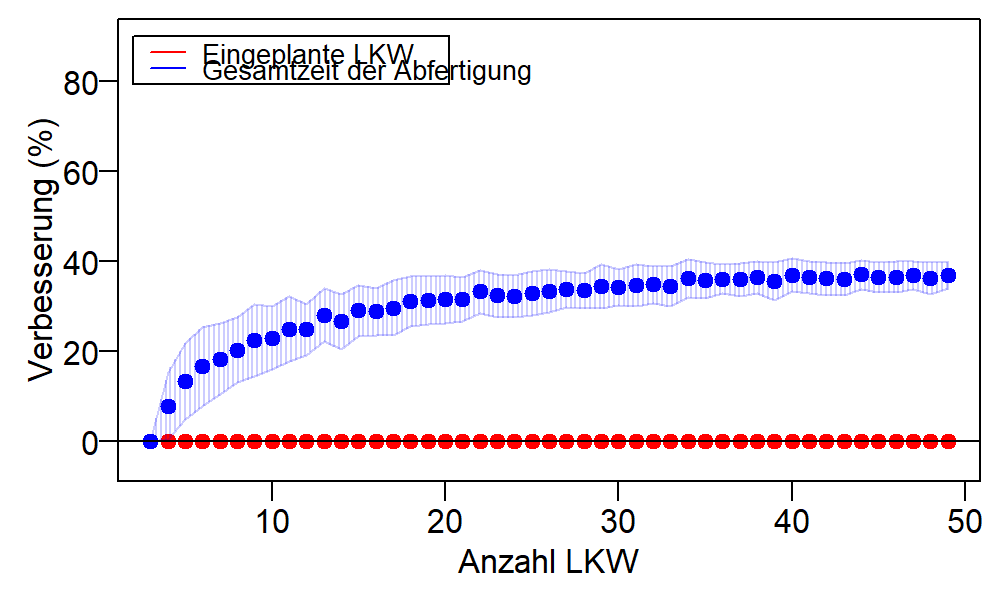
\includegraphics[width=\linewidth]{images/graphs/tspSimulatedAnnealingUnlimited.png}
  \caption{Unbegrenzter Slot}
  \label{fig:etspsimaopt2}
\end{subfigure}
\begin{subfigure}{.495\textwidth}
  \centering
  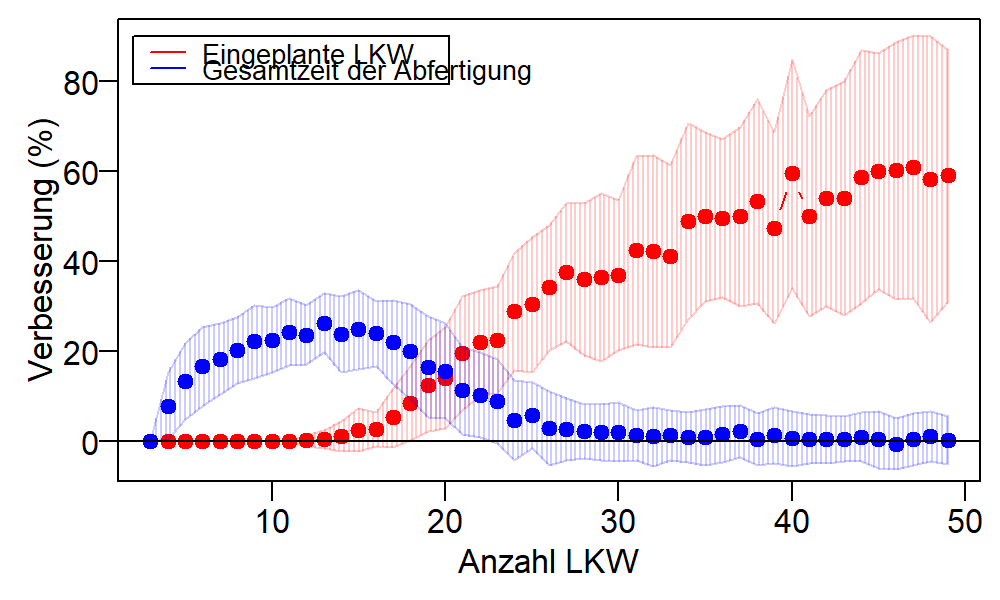
\includegraphics[width=\linewidth]{images/graphs/tspSimulatedAnnealingLimited.png}
  \caption{3 Stunden Slot}
  \label{fig:etspsimaopt2}
\end{subfigure}
\caption{Verbesserung der Abfertigungszeit}
\label{fig:evalTspSimAOpt}
\end{figure}

\todo{Time to complete darstellen?; Punkte weg, nur linie}

Zunächst einmal ist an den Ergebnisgraphen zu erkennen, dass mit dem hier untersuchten Algorithmus definitiv gute Verbesserungen erzielt werden können. Gibt es keine Slotbegrenzung, so können immer alle LKW abgefertigt werden, die rote Linie ist also konstant bei 0, da die Zahl der geplanten LKW in beiden Modellen identisch ist. Die Gesamtzeit, die es braucht, alle LKW zu bearbeiten verbessert sich dagegen. Zunächst einmal steigt diese Verbesserung stark an, sodass bereits bei 10 LKW eine über 20\% kürzere Abfertigungszeit möglich ist. Dann steigt die Verbesserung immer langsamer und nähert sich bis ca. 50 LKW den 40\% an. Die Standardabweichung, also die Streuung der Gesamtabfertigungszeit ist über den gsamten Bereich nicht besonders hoch, verringert sich aber mit streigender Anzahl von LKW noch einmal. Viel interessanter ist allerdings das Verhalten bei begrenztem Slot. Bis ca. 14-15 LKW verhalten sich beide Kurven sehr ähnlich, hier entstehen durch die Slotbegrenzung noch gar keine Einflüsse, im unoptimierten, wie im optimierten Fall können hier noch alle LKW eingeplant werden. Die Verbesserung der Abfertigungszeit erreicht hier auch sein Maximum. Ab dann verbessert sich die Zahl der LKW, welche eingeplant werden können. Im unoptimierten Fall müssen nun langsam die ersten LKW abgewiesen bzw. in andere Slots verschoben werden. Die Zahl der eingeplanten LKW steigt nun sehr stark an und erreicht bei 50 gebuchten LKW knapp 60\% Verbesserung. Allerdings erhöht sich auch die Streuung extrem, d.h. es gibt Fälle in denen deutlich mehr LKW erfolgreich eingeplant werden können, als in anderen. Die Verbesserung der gesamten Abfertigungszeit sinkt ab ca. 15 LKW wieder und nähert sich bei gleichbleibender Streuung der 0 an. Dies liegt daran, dass der Slot in beiden Fällen sehr gut voll ausgelastet wird. Allerdings ist die Zeit pro LKW deutlich geringer, sodass mehr LKW in die gleiche Zeit passen, wie die andere Kurve eben gezeigt hat. 

Insgesamt lässt sich aus diesem Test schlussfolgern, dass mit dem hier getesteten Verfahren durchaus gute Verbesserungen erzielt werden können. Die Höhe der Verbesserung hängt davon ab, wie viele LKW pro Slot gebucht werden dürfen, bzw. ob und in welcher Höhe Überbuchungen erlaubt werden. So hat der Algorithmus mehr Planungsspielraum, es müssten allerdings auch Buchungen auf andere Slots verschoben werden. Um hie die optimale Größe zu finden, wurde das nächste Testszenario durchgeführt.

\subsubsection{Testszenario 5: Verhalten bei Überbuchung}

Wie im vorherigen Szenario festgestellt wurde, hat die Zahl der LKW, welche einen Slot buchen können einen bedeutenden Einfluss auf die Höhe der möglichen Verbesserung. Es stellt sich nun die Frage, ob man eine harte Grenze einführen sollte und keine Buchungen mehr zulässt, wenn die erste Buchung nicht mehr in den Slot passt. Die andere Option wäre es, wie es auch schon für den anderen hier entwickelten Algorithmus empfohlen wurde, eine gewissen Überbuchung zuzulassen. In diesem Fall müssten einige Buchungen zwangsweise im Nachhinein auf spätere Slots verschoben werden. So ergibt sich aber ein noch größerer Spielraum für den Planungsalgorithmus und somit möglicherweise noch weiter verbesserte Abfertigungszeiten. 

Ein entsprechender Testfall wurde in der Testklasse \textit{SimulatedAnnealingTest} in der Methode \textit{test3LoadersBestOf50LimitedOverfill()} implementiert. Der Grundaufbau und die gesammelten Daten sind dabei wie im vorherigen Test. Hier wird allerdings für ein Testreihe die gleiche Liste von Buchungen beibehalten und nur schrittweise eine weitere hinzugefügt. Dies simuliert, dass weitere LKW Fahrer bzw. Speditionen diesen Slot buchen. Dargestellt wird im Auswertungsgraphen dieses mal aber die absolute Zahl von Buchungen, um zeigen zu können, wann nicht mehr alle LKW eingeplant werden können. Eine diagonale Gerade der Steigung 1 zeigt dann des theoretischen Anstieg, ohne begrenzten Slot. Auf einer zweiten y-Achse wird dagegen die Verbesserung der Gesamtkosten aufgetragen, berechnet nach dem gleichen Weg, wie im vorherigen Szenario (siehe Formel \ref{eq:tspCostSaving}).

\begin{figure}[H]
    \centering
    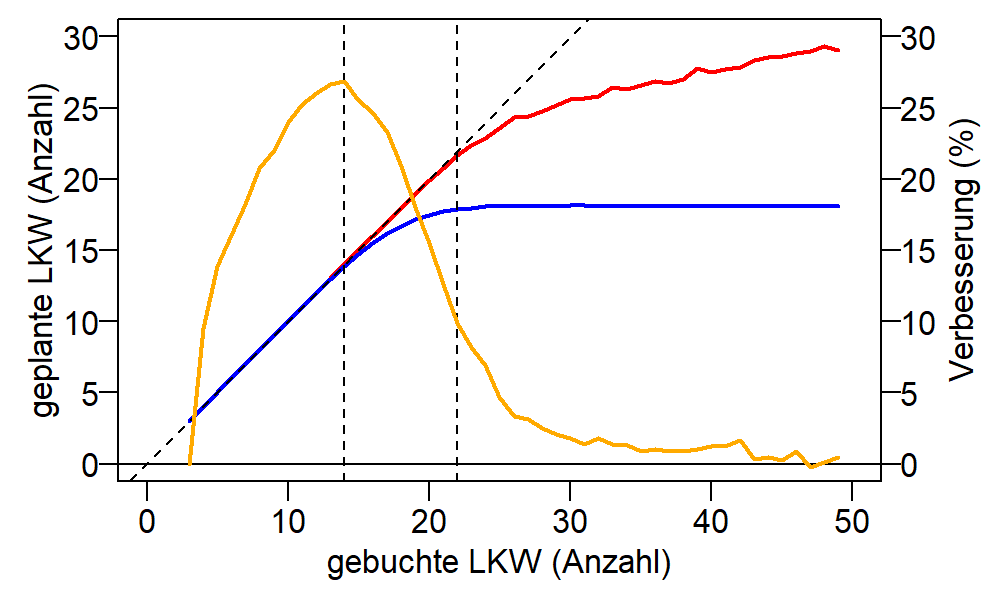
\includegraphics[width=0.7\textwidth]{images/graphs/tspSimALimOverfill.png}
    \caption{Verhalten bei Überbuchung}
    \label{fig:tspEvalOverfill}
\end{figure}

In der Auswertung ist gut zu erkennen, dass selbst bei strikter Begrenzung des Slots eine deutliche Verbesserung möglich ist. Während die blaue Kurve schon bei etwa 14 LKW abfällt und somit zeigt, dass schon nicht immer alle LKW in den Slot passen, fängt die rote, optimierte Kurve erst bei etwa 22 LKW an, langsam abzufallen. Das heißt, selbst wenn bei der Buchung nur so viele LKW zugelassen werden, wie auch in den Slot passen, lassen sich im Durchschnitt schon etwa 8 LKW oder 75\% mehr LKW im Vergleich zum unoptimierten Zustand möglich. Im Vergleich zum unoptimierten Zustand steigt die Zahl der der LKW die geplant werden können kontinuierlich weiter an, d.h. eine Überbuchung würde durchaus noch Verbesserungen bringen. Abzuwägen ist allerdings, wie sich die Verschiebung von nicht mehr passenden Buchungen auf die nächsten Slots auswirkt. Zu vermuten ist, dass die Kategorien der dann verschobenen LKW nicht mehr gleichmäßig sein wird. Da tendenziell eine Sortierung nach Kategorien erfolgt, da diese leicht und schnell nacheinander abzuarbeiten sind, werden Buchungen mit gut passenden Kategorien vermutlich eher eingeplant, während andere Kategorien nicht mehr so gut passen. Wie gut der Algorithmus mit Ungleichverteilungen klar kommt, soll noch in folgenden Tests beurteilt werden \todo{Reihenfolge der Tests?}. Festzuhalten ist aber, dass eine extreme Überbuchung immer weniger Vorteil bringt, sodass man im Beispiel höchstens Größenordnungen von insgesamt ca. 30 gebuchen und somit etwa 25 geplanten LKW überbuchen sollte. Dies entspricht einer Überbuchung von ca. 30-40\%. Hier ist die Steigung noch vergleichsweise größer.

\todo{Kostenverbesserung (gelbe Kurve) beschreiben und bewerten}

\subsubsection{Testszenario 6: Variation von Parametern}

% Verhalten bei unterschiedlicher Slotgröße
% Unterschiedliche Anzahl von Landeplätzen
% Ungleiche Verteilung der Kategorien

Bisher wurde der Algorithmus auf sein Verbesserungspotenzial bei in als gewöhnlich angenommenen Fällen untersucht. In dieser Testreihe soll nun auch wieder der grunsätzliche Testablauf auf Szanario 4. Es soll also immer die prozentuale Verbesserung, der Zahl der eingeplanten LKW gegenüber der Zahl an gebuchten LKW dargestellt werden. Eine Reduzierung der Abfertigungszeit pro LKW und somit Erhöhung der möglichen LKW war oberstes Ziel der Optimierung. Dargestellt werden in jedem Testfall pro Graph einige beispielhafte Verläufe, bei Variation des jeweils getesteten Parameters.

\textbf{Slotgröße}


Der erste wichtige Parameter ist die Größe der Slots, auf die die LKW aufgeteilt werden müssen. Eine stärkere Begrenzung auf kürzere Zeiträume würde für die LKW Fahrer eine genauere Planung erlauben. Gleichzeitig gibt es aber in größeren Slots auch mehr Spielraum für die Verteilung der LKW. Mit dem hier durchgeführten Test soll gezeigt werden, welche Slotgröße im Bezug auf die mögliche Verbesserung der Anzahl möglicher LKW am geeignetsten ist. Ausgewertet wurden hier beispielhaft Slots der Größen 1, 2, 4 und 6 Stunden, da dies realistisch vorstellbare Größen für einen Arbeitstag wären.

\begin{figure}[H]
    \centering
    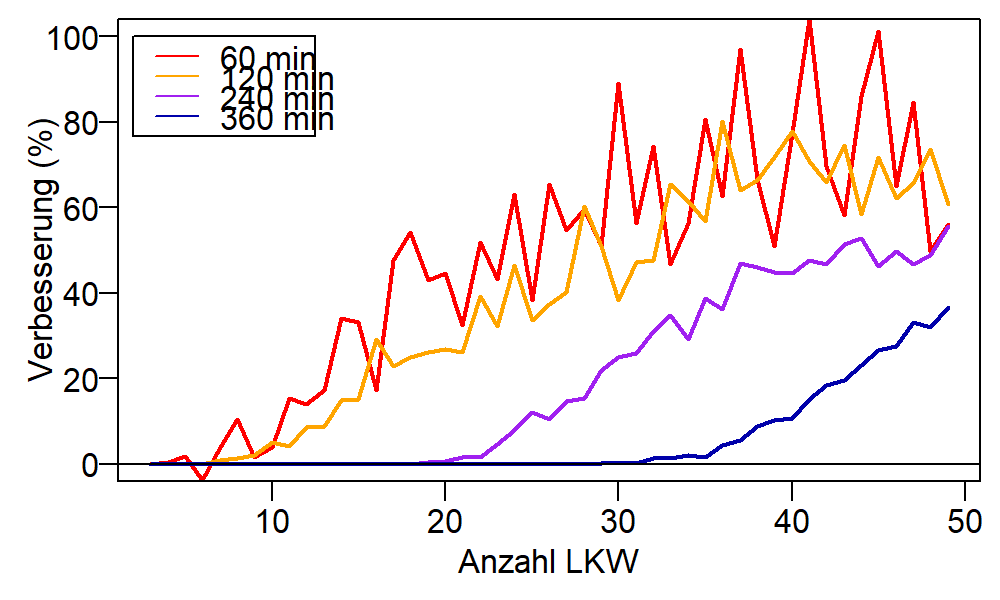
\includegraphics[width=0.7\textwidth]{images/graphs/tspSimALimSlotsize.png}
    \caption{Verhalten bei unterschiedlicher Slotgröße (test3LoadersBestOf50LimitedSlotsize(), tspSlotsize.R)}
    \label{fig:tspEvalSlotsize}
\end{figure}

\todo{Evtl. bis 100 LKW}

Was in dem Auswertungsgraphen zu erkennen ist, ist dass sich die Verbesserung für alle Slotgrößen im Mittel auf maximal 60-70\% Verbesserung einpendelt \todo{Mit längerem Graphen verifizeiren}. Je größer der Slot ist, desto länger dauert dies natürlich, mehr LKW hineinpassen und eine gewisse Überbuchung notwendig ist. So erkennen ist aber auch, dass schon die Durchschnittswerte extrem schwanken, je kleiner der Slot ist. In einigen Fällen lässt sich dort eine sehr gute Verbesserung erzielen, in anderen aber auch eine sehr viel weniger Gute. Erklären lässt sich das vermutlich damit, dass ein kleiner Slot einfach sehr begrenzt ist. Der Spielraum bei der Optimierung ist wesentlich geringer und die \glqq{}Ketten\grqq{} von LKW, welche gleiche oder ähliche Kategorien haben und somit alle nacheinander mit dem gleichen Ladehilfmittel abgefertigt werden können, sind einfach wesentlich kürzer. Es sind zwangsweise mehr Hilfsmittelwechsel, spätestens zum Anfang und Ende des Slots nötig. Aus dieser Betrachtung heraus kann man also sagen, dass größere Slots tendenziell besser sind. Mit einer entsprechend auch höheren Anzahl von Buchungen lassen sich ähnlich hohe Verbesserungen erzielen, deren Höhe ist allerdings wesentlich konstanter und weniger schwankend. Hier ist eine Abwägung zwischen Bedürfnissen des Terminals und der LKW Fahrer nötig.


\textbf{Anzahl von Ladeplätzen}

Ebenfalls ist es interessant, wie sich der Algorithmus verhält, wenn die Zahl der Ladeplätze variiert wird. Auch wenn dies vermutlich kein Parameter ist, auch den die Entwickler einen großen Einfluss haben und der vermutlich vom Terminal vorgegeben ist, so kann es doch zumindest interessant sein, das Verhalten des Algorithmus in dieser Situation zu kennen. Ausgewertet wurde im folgenden die Anzahlen 1, 3, 5 und 10 der Ladeplätze, was einige beispielhafte Werte darstellt, die vermutlich in dieser Größenordnung in der Realität vorkommen.

\begin{figure}[H]
    \centering
    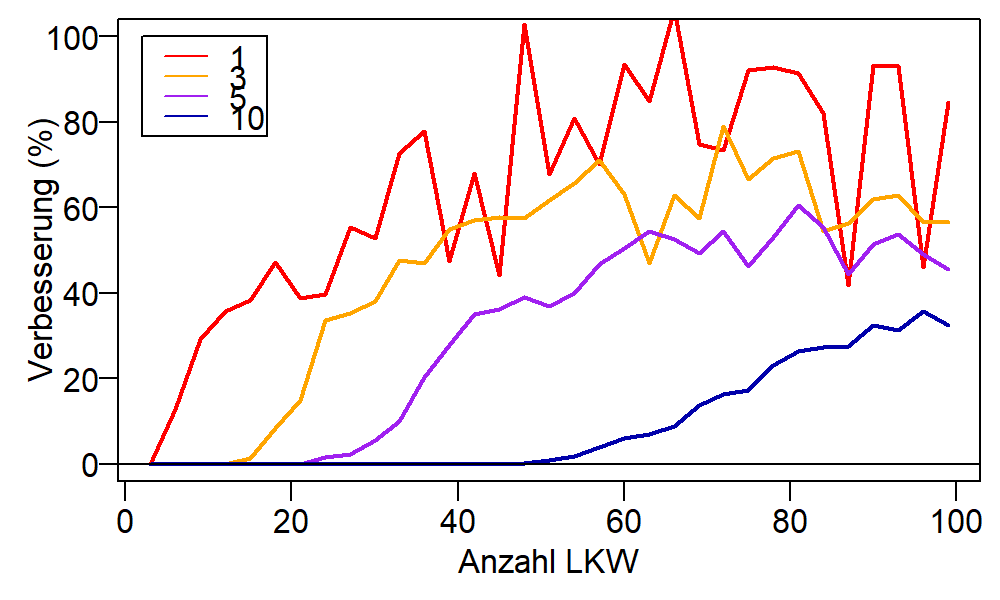
\includegraphics[width=0.7\textwidth]{images/graphs/tspSimALimLoaders.png}
    \caption{Verhalten bei unterschiedlicher Anzahl von Ladeplätzen (test3LoadersBestOf50LimitedLoaders(), tspLoaders.R)}
    \label{fig:tspEvalLoaders}
\end{figure}

Bei der Änderung der Anzahl von Ladeplätzen lassen sich ganz ähnliche Beobachtungen machen, wie auch schon bei Änderung der Slotgröße. Der Anstieg ist bei kleinerer Anhal von Plätzen natürlich zunächst höher, da auch insgesamt weniger LKW hinein passen. Allerdings geht die relative Verbesserung auch hier wieder in ähnlich hohe Regionen. Es ist auch wieder zu erkennen, dass die Schwankung bei wenigen Slots extrem hoch ist und mit steigender Anzahl deutlich geringer wird. Die Durchschnittskurven sind hier deutlich gleichmäßiger. Auch hier dürfte das mit dem Planungsspielraum zusammenhängen, da die Buchungen einfach auf mehr Plätze aufgeteilt werden können und so auf jedem Platz weniger Wechsel zwischen den Ladekategorien und -hilfsmitteln stattfindet. Im Endeffekt sind also auch hier wieder mehr Ladeplätze besser geeignet für eine gleichmäßige Verteilung, auch wenn im allgemeinen Durchschnitt in allen Varianten ähnlich viele LKW bearbeitet werden können.


\textbf{Ungleiche Verteilung der Ladekategorien}






\subsection{Vergleich der Lösungen}




\subsubsection{Fazit Algorithmus 1}

Nach der Durchführung der Testszenarien zum Vergleich der verschiedenen Planungsverfahren haben sich tatsächlich erstaunliche Ergebnisse ergeben. Ausgewählt wurden die betrachteten Verfahren bei der Planung, da sie bestimmten Heuristiken folgen, welche in der Theorie als sinnvoll und vor allem besser geeignet als das bisherige, unoptimierte Vorgehen erschienen. Es hat sich aber gezeigt, dass sich nicht alle Verfahren in der Praxis so verhalten, wie es in der Planung vermutet wurde. Dies war aber auch genau das Ziel dieser Auswertung.

Alle Verfahren teilen sich das Problem, dass sie relativ große Schwankungen und Streuungen in der Qualität der Ergebnisse aufweisen. Da dies bei allen Verfahren teils mehr, teils etwas moderater auftritt, lässt sich vermuten, dass dies zum großen Teil auch auf Einsatzsituation zurückzuführen ist. Es lässt sich leider nicht vermeiden, dass die Eingangsdaten einer relativ großen Willkür und Zufälligkeit unterliegen. Sicherlich ließe sich diese etwas minimieren, indem noch genauere Analysen, beispielsweise zur Verteilung und relativen Anzahl der Abfertigungskategorien zueinander angestellt würden. Eine allgemeingültige Lösung ist deutlich schwieriger zu optimieren, dies ist aber im betrachteten Kontext auch nicht unbedingt anders möglich. Das reale Problemfeld ist nun einmal sehr unübersichtlich und komplex, mit Einschränkungen und Annahmen lässt sich dies nur bedingt sinnvoll ändern.

Insbesondere das SJN Verfahren hat sich nicht besonders tauglich als allgemeine Lösung gezeigt. Es ist einfach sehr stark davon abhängig, welche Aufgaben wie lange brauchen. Für einige Fälle mag dieses Verfahren gut funktionieren, aber in vielen Fällen wird es Abfertigungskategorien geben, welche immer schneller gehen als andere, wodurch es einseitige Verteilungen gibt. Die schnellere Abfertigung und geringere Wartezeit ist sicherlich ein Vorteil dieses Ansatzes, dies war aber nicht Hauptaugenmerk der Optimierung und bringt schlussendlich auch gar keine allzu großen Vorteile. Die Idee einer festen Planung war es nämlich auch, den LKW Fahrern feste Zeitpunkte nennen zu können, in denen sie ankommen sollen. Ob diese nun zu Beginn nah beieinander liegen oder sehr verteilt ist dann irrelevant. Die beiden anderen Verfahren MIT und FCFS sind sich dagegen wesentlich ähnlicher als angenommen. Die Vorteil, welcher in der Planung im MIT Verfahren gesehen wurde war, dass die Auslastung deutlich besser wird, wenn zunächst Aufgaben verplant werden, welche wenig genutzte Ressourcen benötigen. Das FCFS Verfahren war zusätzlich eher als interessanter Vergleich gedacht, wie sich eine ganz zufällige Verteilung auswirkt. Aus der Ähnlichkeit der Ergebnisse lässt sich schlussfolgern, dass dieser Gedanke gar nicht so entscheidend für das Ergebnis ist. Vielmehr scheint es, gerade im Vergleich zum SJN Verfahren zu bringen, die Aufgaben aus unterschiedlichen Kategorien gleichmäßig zu verplanen. Dies scheint die Leerlaufzeiten schon sehr gut auszufüllen. Insbesondere das FCFS Verfahren zeigt bei der Verbesserung der Anzahl von abgefertigten LKW (siehe Abb. \ref{fig:eal3}) eine größere Steigerung als beim MIT Ansatz. Auch hier wird eine relativ gleichmäßige Verteilung der Kategorien durch das Planen der weniger genutzten Ressourcen erreicht. Interessanterweise ist allerdings eine komplett zufällige Planung in diesem Fall immer noch ein kleines bisschen besser. 

Den allergrößten Optimierungsvorteil scheint man allerdings schon ganz einfach dadurch erreichen zu können, dass man den LKW Fahrern feste Zeitpunkte zuweist und eben keine zufällige Ankunft innerhalb des Slots ermöglicht. So lässt sich viel konkreter und mit viel weniger Unsicherheit eine Planung erstellen. 
Insbesondere die Leerlaufzeiten zwischen den Aufträgen lassen sich dadurch bei allen Verfahren stark minimieren (Abb. \ref{fig:evalLeerlaufzeit}) und eine gezieltere Auslastung der Ressourcen kann erreicht werden.

Will man aus dieser Evaluation nun auf ein Verfahren festlegen, welches weiter genutzt werden sollte, so wäre dies der FCFS Ansatz. In Kombination mit einer moderaten Überbuchung lassen sich hier durchaus gut verbesserte Planungen erzeugen, was die Anzahl der bearbeiteten LKW und auch die Leerlaufzeiten angeht. Eine möglichst gute Verteilung der Ressourcen ist im Vorhinein definitiv gut und trägt zu noch besseren Ergebnissen bei, eine Verbesserung lässt sich aber auch bei moderaten Ungleichverteilungen erzielen.

\subsubsection{Fazit Algorithmus 2}

Zunächst einmal kann man festhalten, dass es in dieser Evaluation im Gegensatz zum anderen Algorithmus in erster Linie nicht um die Bewertung verschiedener Verfahren innerhalb der Implementierung ging. Dort wurde der Effekt verschiedener heuristischer Ansätze untersucht. Hier ist es dagegen so, dass das zugrunde liegende Traveling Salesman Problem zumindest theoretisch immer perfekt gelöst werden kann. Zu Beginn ging es in den drei Testszenarien also eher darum, eine Einschätzung zu geben, wie geeignet die drei beispielhaft implementierten Lösungsverfahren für das TSP sind. Dabei hat sich schnell herausgestellt, dass die beiden exakten Branch and Bound bzw. Reduced Matrix Verfahren zumindest in der hier implementierten Form nicht geeignet sind, um die für die Problemstellung benötigten Graphen zu lösen. Für das Simulated Annealing Verfahren konnte gezeigt werden, dass es spätestens nach mehreren Durchläufen zumindest nahezu das perfekte Ergebnis liefert. Somit war das Finden eines geeigneten Lösungsverfahrens zwar ein wichtiges Ziel dieser Evaluation, unter der Annahme, dass alle Verfahren das gleiche und beste Ergebnis liefern, sind die anschließenden Testszenarien allerdings unabhängig vom eigentlichen Lösungsverfahren gültig und zeigen allgemein wie gut der Ansatz ist, das in der Arbeit betrachtete Problem mit Hilfe des Traveling Salesman Problems lösen.

%Lösungsverfahren
Bezüglich der Lösungsverfahren lässt sich festhalten, dass grundsätzlich alle geeignet erscheinen, das TSP und somit auch die vorliegende Problemstellung zu lösen. Insbesondere die beiden exakten Verfahren zeigen aber einen sehr großen Zeit bzw. Rechenressourcen-Bedarf mit steigender Zahl von Knoten im zu lösenden Graphen. Dies war auch schon nach der theoretischen Betrachtung zu erwarten, allerdings wurden die Grenzen noch schneller erreicht, als vermutet. Theoretisch sollten die Verfahren für Graphen mit etwa xyz Knoten geeignet sein\todo{Zahl und Quelle heraussuchen}. Wie die Versuche gezeigt haben hängt diese Größe auch sehr von den zur Verfügung stehenden Rechenressourcen ab. Ein weiterer wichtiger Aspekt ist aber wahrscheinlich die Implementierung der Verfahren. Durch die Umsetzung einer wesentlich effizienteren und Zeit- bzw. Ressourcensparenderen Lösung, möglicherweise sogar in einer für solche Rechenoperationen besser geeigneten Programmiersprache als Java, ist hier sicherlich noch viel Potenzial herauszuholen. In der Gegebenen Zeit dieser Arbeit war es nicht möglich und auch nicht das Ziel, hier ein perfektes und hoch optimiertes Verfahren zu implementieren. Viel mehr sollte gezeigt werden, dass die Planung und der allgemeine Ansatz zur Lösung des vorliegenden Problems geeignet und umsetzbar sind. Dazu haben die hier genutzten, rudimentären Implementierungen vollkommen ausgereicht. Sollte man diesen Ansatz weiter verfolgen wollen und ihn in einer realen Implementierung einsetzen, dann kann der modulare Aufbau des Java-Projekts genutzt werden und eine entsprechend verbesserte oder sogar ganz andere Implementierung eingesetzt werden. Für die weitere Analyse bietet der Simulated Annealing Ansatz allerdings eine gute Basis. Unter Verwendung der optimierten Parameter und durch wiederholtes Durchlaufen des Algorithmus lässt sich eine nahezu perfekte Lösung bei sehr geringem Rechenzeitbedarf erzielen. Selbst wenn sich ein noch besseres Verfahren implementieren ließe, würde dies die anschließenden Auswertungen nur noch etwas weiter verbessern.

%Bewertung effektivität des algorithmus
Zu dem Algorithmus selbst lassen sich aus den Testszenarien, aber auch aus den Erfahrungen aus der Planung und Implementierung einige Schlussfolgerungen ziehen. Zunächst einmal konnte gezeigt werden, dass sich auch im praktischen Einsatz eine gute Optimierung erzielen lässt. Die Dauer der Abfertigung einzelner LKW kann verringert werden, wodurch bei weiterer Füllung eines Slots 40-60\% mehr LKW eingeplant und bearbeitet werden können. Eine Überbuchung der Slots scheint hier im Gegensatz zum anderen Algorithmus nur bedingt sinnvoll und muss im realen Einsatz genau abgewogen werden. Insgesamt funktioniert das hier genutzte Verfahren am besten und arbeitet am effektivsten, wenn ein gewisser Planungsspielraum gelassen wird, d.h. wenn eine gewisse Slotgröße und eine gewisse Zahl an Ladeplätzen vorhanden ist. So lässt sich einfach die beste Verteilung der LKW erzielen. Ein Nachteil der Nutzung des Traveling Salesman Problems, insbesondere des mTSP für mehrere Ladeplätze ist es, dass hier zwar die insgesamt die kürzeste Bearbeitungsdauer ermittelt wird, dadurch entsteht aber auf die einzelnen Plätze bezogen nicht zwangsweise eine gleichmäßige Verteilung. Die Lösung, welche hierfür geplant und umgesetzt wurde ist, dass zunächst eine Aufteilung auf unbegrenzte Slots erfolgt und dann eine Limitierung bzw. Umverteilung erfolgt, sodass alle Ladeplätze für die Zeit des Slots so gut wie möglich ausgelastet sind. Dieses Vefahren wurde schon so geplant, dass eine möglichst effektive Reihenfolge bestehen bleibt, das best mögliche Ergebnis entsteht dadurch aber vermutlich nicht. Dies war aber die Einschränkung, welche in Kauf genommen wurde, da hier nun einmal das mTSP als Ansatz genutzt wurde, welches eben die insgesamt besten Kosten und nicht die beste Verteilung zum Ziel hat. Insgesamt sind die Auswertungen eher als Nachweis zu sehen, dass die Idee grundsätzlich funktionieren kann. Es wurden allgemein sehr viele Annahmen getroffen, insbesondere auch was den Zeitbedarf der Abfertigung bestimmter Güter angeht. Mit anderen Werten, welche sich in einem realen Einsatz ergeben werden, könnten hier sicherlich noch etwas andere Zahlen herauskommen. Es lassen sich außerdem teils sehr große Schwankungen und Streuungen in den Ergebnissen erkennen. Wie schon im anderen Algorithmus geschlussfolgert wurden, ist es auch hier so, dass eine relativ große Willkür und Zufälligkeit bei den Eingangsdaten besteht. Dies wurde an die Praxis angelehnt und lässt sich auch da nicht vermeiden, sodass es allgemein sehr schwierig ist, konstant gute oder gleich gut Verbesserte Ergebnisse zu erzielen. Das liegt einfach in der Natur der Problemstellung.

Das Fazit zu diesem Algorithmus ist also, dass die Idee, eine möglichst kurze Abfertigungszeit zu erzielen, indem man schau, welche LKW am schnellsten nacheinander bearbeitet werden können, durchaus funktioniert. Setzt man ein passendes Lösungsverfahren für das TSP ein, so können sichtbar verbesserte Zeitplanungen erzeugt werden.


\subsubsection{Vergleich der Algorithmen}

Ein direkter, vor allem quantitativer Vergleich der beiden Algorithmen ist kaum sinnvoll möglich. Beide sind in ihren konzipierten Einsatzbereichen geeignet und können verbesserte Ergebnisse erzielen. Allerdings sind die Ansatzpunkte und der Fokus beider Algorithmen durchaus verschieden. Auch die verwendeten Zeiten, insbesondere die angenommenen Abfertiungszeiten pro Kategorie basieren auf Annahmen aus der vorherigen Analyse und sind kaum direkt miteinander zu vergleichen. Welches Optimierungskonzept schlussendlich eingesetzt werden sollte, hängt also vermutlich eher von den schlussendlichen, realen Anforderungen ab und wie sich diese in die Praxis integrieren lassen.


\subsection{Gesamtbewertung}

Nachdem nun die zu Beginn gestellte Problemstellung ausführlich analysiert, geplant, implementiert und bewertet wurde, sollen an dieser Stelle noch einmal alle Erkenntnisse zusammengefasst werden. Über den ganzen Entwicklungsprozess konnten mit Blick auf die bearbeitete Problematik sehr viele Aspekte und Erkenntnisse gewonnen werden. Der ganze Prozess diente dazu, eine prototypische Optimierung des gegebenen Problems zu Entwickeln und auf dem Wege Erkenntnisse bezüglich einer möglichen Lösung zu erlangen und zu erarbeiten. 

Schon bei der Analyse ist dabei aufgefallen, dass die Ausgangssituation und damit auch eine potenzielle Lösung durchaus komplex und nicht trivial und geradlinig umzusetzen ist. Es mussten schon zu Beginn der Planungsphase Ideen entwickelt werden, wie all diese Aspekte in ein Verfahren bzw. einen Algorithmus überführt werden können, welcher dann als Software implementiert werden kann. Bei der Recherche zeigte sich schnell, dass es der einzig wirklich erfolgversprechende Weg ist, bestehende Verfahren mit bereits zumindest teilweise vorhandenen Lösungsansätzen einzusetzen. Es sind einfach so viele Parameter und Einschränkungen zu bedenken, dass anders keine sinnvolle und vor allem in dem gegebenen Zeitrahmen erfolgversprechende Lösung zu erreichen war. Es hat sich allerdings ebenfalls schnell herausgestellt, dass auch die Nutzung von bereits bekannten Verfahren diverse Probleme mit sich bringt. Eine direkte Adaption auf das hier gegebene Problem mit all seinen Facetten ist auch hier nicht möglich. Es war also nötig, die Problemstellung durch passende Einschränkungen so zu formen, dass fertige Verfahren zur Lösung angewendet werden können. Um hier einen Spielraum zu haben und unter den Bedingungen eine geeignete Lösung finden zu können wurden die zwei Algorithmen parallel implementiert. Beispielsweise die Nutzung des Traveling Salesman Problems wurde schnell als scheinbar gut passende Lösung gefunden. Das Finden einer optimalen Reihenfolge für möglichst geringe Kosten und bereits gut bekannte Lösungsverfahren erscheinen zunächst als sehr guter Ausgangspunkt, allerdings zeigte sich auch hier bei genauerer Betrachtung, dass Einschränkungen wie begrenzte Slots nur unter Umwegen adaptierbar sind. Allerdings mussten einige Anforderungen, wie möglicherweise verschiedene nutzbare Geräte für eine Abfertigungskategorie, hier weg abstrahiert werden, um überhaupt die Chance auf eine funktionierende Lösung zu haben. Auch bei dem anderen Verfahren, welches versucht, einen Zeitplan über Heuristiken zu erstellen, haben sich solche Probleme aufgetan. Hier konnte der Aspekt mit Wechselzeiten und entsprechenden Optimierungen durch passende Reihenfolge nicht berücksichtigt werden, ansonsten wäre es auch hier sehr schwer gewesen, sinnvolle Ergebnisse unter Berücksichtigung aller Anforderungen zu erzielen.

Der hohen Zahl von Einschränkungen und Anforderungen an ein mögliches Ergebnis stehen immer die eher Willkürlichen und wenig planbaren Eingabedaten gegenüber. Dadurch, dass die LKW in Ankunftszeit und Warenart aus Terminal sich sehr zufällig und wenig planbar kommen, ist auch eine gute Planung sehr schwer zu realisieren. Dadurch zeigt sich auch in vielen der vorangegangenen Auswertungen eine hohe Streuung und Variabilität in den Ergebnissen. Es gibt Fälle, in denen sehr gute Verbesserungen erzielt werden können, genau so gut kommt es aber auch oft vor, dass die prozentuale Verbesserung sehr gering ausfällt. In der Ausgangssituation kommen LKW innerhalb ihres gebuchten Slots an, wann sie wollen. Diese Praxis beizubehalten ist nicht möglich, wenn in irgendeiner Form eine sinnvolle Vorausplanung erzeugt werden soll. Es hat sich über die ganze Entwicklung gezeigt, dass eine optimale Abfertigung nur möglich ist, wenn ein konkreter Zeitplan erstellt wird, der für jeden LKW genaue Zeiten festlegt und der so auch eingehalten werden muss. Ohne eine feste Taktung können einfach die Potenziale zur Zeitersparnis nicht ausgenutzt werden. Ein realer Einsatz der hier entwickelten Algorithmen setzt also grundsätzlich voraus, dass diese Zeitplanung auch praxistauglich ist. LKW Fahrer müssten also vorab einen Slot in festzulegender Größe buchen, im späteren Verlauf wird ihnen nach abgeschlossener Zeitplanung eine feste Uhrzeit mitgeteilt, zu der sie sicher am Terminal erscheinen müssen. Durch hinzufügen von Pufferzeiten ließe sich hier sicherlich noch ein gewisser Spielraum erzeugen, aber Verschiebungen innerhalb des Zeitplans durch z.B. Stau oder welche Gründe auch immer durch die perfekt getaktete Reihenfolge nicht möglich \todo{Expertenmeinung dazu?!}. Es stellt sich also die Frage, ob Speditionen und LKW Fahrer ein solches Modell akzeptieren würden und vor allem ob sie dies auch einhalten können. Gibt es zu viele Ausfallzeiten durch verspätete LKW ist das ganze Modell für das Terminal auch hinfällig und nicht 
nutzbar. Eine weitere Unsicherheit in einem solch eng getakteten Zeitplan ist, wie genau die Schätzung der Abfertigungszeiten bzw. der Maschinenwechselzeiten wirklich möglich ist. Sicherlich ließen sich hier noch komplexere Berechnungen implementieren, aber eine genaue Schätzung könnte bei einer derart hohen Variablität von Waren durchaus schwierig werden. Setzt man hier zu hohe Pufferzeiten ein, sinkt das Optimierungspotenzial stark, zu gering geschätzte Zeiten bringen allerdings den ganzen Zeitplan durcheinander und haben große Auswirkungen auf alle nachfolgenden LKW. 





%- Hohe Schwankungen
%- Schwierige Vorhersage
%- Festlegung von Zeiten unumgänglich für eine Optimierung

%- Diskussion Praxistauglichkeit

%- Allgemein Feste Zeiträume nach Kategorie so gut schätzbar und in der Praxis sinnvoll?

%- Viele Aspkete abstrahiert und in den algos nicht berücksichtigt

%- Schwer mit vorgefertigten Verfahren in so einem konkreten Problem zu arbeiten

%- Fokus musste auf bestimtme Askepkte pro Algo gelegt werden



\todo{Richitge stelle?
Diskussion: Einbettung des Ganzen in eine reale Anwendung. 
 - Wie/Wo sloteingabe, welcher Slot auswählbar, was bei Verschiebungen?, Benachtigungen, Priokunden, ...}
